\documentclass[a4paper]{article}

% CJK support: prefer ctex, fallback to XeTeX native line breaking
\IfFileExists{ctex.sty}{
  \usepackage[fontset=fandol]{ctex}
}{
  % Fallback for minimal TeX installs (e.g. MacTeX Basic, TeX Live scheme-basic)
  % without ctex/xeCJK. Uses XeTeX's built-in CJK line breaking.
  \usepackage{fontspec}
  \XeTeXlinebreaklocale "zh"
  \XeTeXlinebreakskip = 0pt plus 1pt
  \IfFontExistsTF{Songti SC}{\setmainfont{Songti SC}}{%
    \IfFontExistsTF{Noto Serif CJK SC}{\setmainfont{Noto Serif CJK SC}}{}%
  }
  \IfFontExistsTF{Heiti SC}{\setsansfont{Heiti SC}}{%
    \IfFontExistsTF{Noto Sans CJK SC}{\setsansfont{Noto Sans CJK SC}}{}%
  }
}

% Basic packages
\usepackage{amsmath, amssymb}
\usepackage{graphicx}
\usepackage[margin=2.5cm]{geometry}
\emergencystretch=3em
\usepackage[most]{tcolorbox}
\usepackage{etoolbox}
\usepackage{listings}
\usepackage{hyperref}
\usepackage{booktabs}
\usepackage{array}
\usepackage{subcaption}
\usepackage{float}
\usepackage{tikz}
\IfFileExists{pgfplots.sty}{
    \usepackage{pgfplots}
    \pgfplotsset{compat=1.18}
}{}

% ===== Highlight boxes =====
\newtcolorbox{knowledgebox}[1]{
    enhanced, colback=blue!5!white, colframe=blue!75!black, colbacktitle=blue!75!black,
    coltitle=white, fonttitle=\bfseries, title={#1}, attach boxed title to top left={yshift=-2mm, xshift=2mm},
    boxrule=1pt, sharp corners
}

\newtcolorbox{importantbox}[1]{
    enhanced, colback=yellow!10!white, colframe=yellow!80!black, colbacktitle=yellow!80!black,
    coltitle=black, fonttitle=\bfseries, title={#1}, sharp corners
}

\newtcolorbox{warningbox}[1]{
    enhanced, colback=red!5!white, colframe=red!75!black, colbacktitle=red!75!black,
    coltitle=white, fonttitle=\bfseries, title={#1}, sharp corners
}

\newtcolorbox{practicebox}[1]{
    enhanced, colback=black!3!white, colframe=black!75, colbacktitle=black!75,
    coltitle=white, fonttitle=\bfseries, title={#1}, sharp corners
}

% ===== Code listings =====
\lstset{
    basicstyle=\ttfamily\small,
    keywordstyle=\color{blue},
    stringstyle=\color{red!60!black},
    commentstyle=\color{green!60!black},
    breaklines=true,
    frame=single,
    numbers=left,
    numberstyle=\tiny\color{gray},
    captionpos=b,
    extendedchars=false
}

% ===== Figure provenance and unit macros =====
% \vtag goes inside \caption{...}; \srcnote{MM:SS--MM:SS} follows the figure environment.
\newcommand{\vtag}{\protect\footnotemark}
\newcommand{\srcnote}[1]{\footnotetext{视频画面时间区间：#1。若为裁剪图，时间区间仍对应原视频画面。}}
% Units work in text and math mode; never hand-write $^\circ$ or \AA inside \mathrm.
\newcommand{\degC}{\ensuremath{^{\circ}\mathrm{C}}}
\newcommand{\um}{\ensuremath{\mu\mathrm{m}}}
\newcommand{\nm}{\ensuremath{\mathrm{nm}}}
\newcommand{\angstrom}{\ensuremath{\text{\AA}}}

% ===== Front-page metadata =====
% Fill these in when generating notes.
\newcommand{\notetitle}{我解开了华容道}
\newcommand{\notesubtitle}{滑动积木的状态图：从格子到 25955 个节点}
\newcommand{\noteauthors}{根据 2swap 视频整理}
\newcommand{\notedate}{2025年8月22日}
\newcommand{\videochannel}{2swap}
\newcommand{\videopublishdate}{2025年8月22日}
\newcommand{\videoduration}{12分19秒}
\newcommand{\videourl}{https://www.youtube.com/watch?v=YGLNyHd2w10}
\newcommand{\videocoverpath}{cover.jpg}

\begin{document}

% ===== Title page =====
\begin{titlepage}
\centering
{\Large 课程笔记\par}
\vspace{1.2cm}
{\huge\bfseries \notetitle\par}
\ifdefempty{\notesubtitle}{}{
\vspace{0.3cm}
{\large \notesubtitle\par}
}
\vspace{0.5cm}
{\large \noteauthors\par}
\vspace{0.3cm}
{\large \notedate\par}
\vspace{1.0cm}

\ifdefempty{\videocoverpath}{
{\small 请在生成笔记时填入视频封面图的本地路径。\par}
}{
\includegraphics[width=0.82\textwidth,height=0.40\textheight,keepaspectratio]{\videocoverpath}\par
}

\vfill
\begin{tcolorbox}[width=0.9\textwidth, colback=black!2!white, colframe=black!60, sharp corners]
\textbf{视频作者/频道}：\videochannel\par
\textbf{发布日期}：\videopublishdate\par
\textbf{视频时长}：\videoduration\par
\textbf{视频链接}：
\ifdefempty{\videourl}{
未填写
}{
\href{\videourl}{\nolinkurl{\videourl}}
}
\end{tcolorbox}
\end{titlepage}

\tableofcontents
\newpage

%% --- 正文内容开始 --- %%

\section{滑动积木的盘面，为什么要用图来记？}

讲者开场放出的，并不是一个人在缓慢试步，而是一个随机智能体，正在华容道（Klotski）的状态空间里四处游走。左上角是一盘彩色滑块，右侧是已经探访过的状态织成的细网。这类积木谜题随处可见，但讲者要强调的不是“怎么过关”，而是：这些可以滑动的块一旦被允许或禁止某些位移，它们本身就定义了一张图。图的局部有曲折的子结构，整体又有更大的超结构。

\noindent\begin{minipage}{\textwidth}
\begin{figure}[H]
\centering
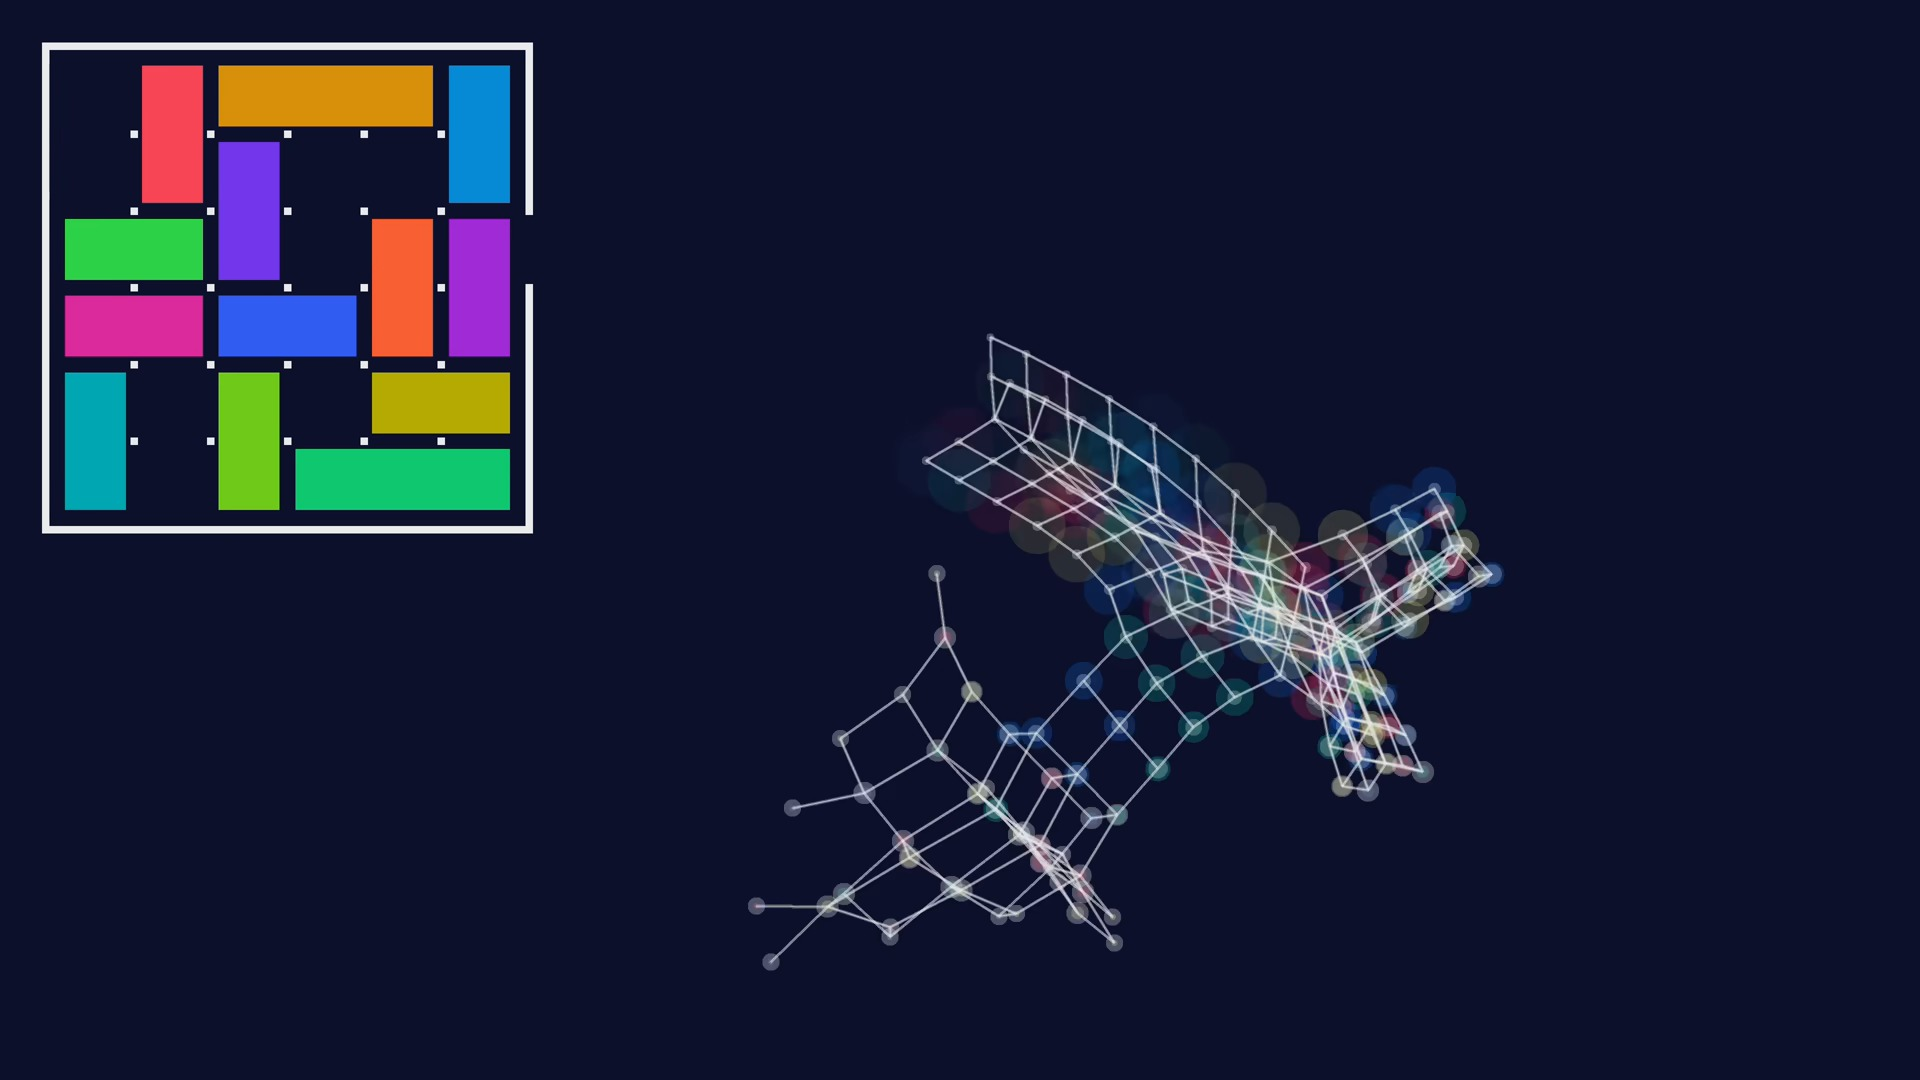
\includegraphics[width=0.90\textwidth]{figures/fig_01_klotski_intro.jpg}
\caption{随机智能体正在探索华容道的状态空间：左侧是当前盘面，右侧是已经走访过的状态构成的图\vtag}
\end{figure}
\srcnote{00:00:00--00:00:19}
\end{minipage}

常见的入门盘面是一块 $6\times 6$ 的格子，目标是把某块积木从右侧的开口里“放出去”。眼前这块还出不去，因为出口被另一块挡住了。要把这种局面说清楚，讲者采用最朴素的图论语言：把当前盘面记成一个节点；若只滑动一次就到达另一种盘面，这两个节点之间就连一条边。一种局面往往只和少数几种邻居相连，边一层层延伸出去，便成为迷宫般的道路。

\noindent\begin{minipage}{\textwidth}
\begin{figure}[H]
\centering
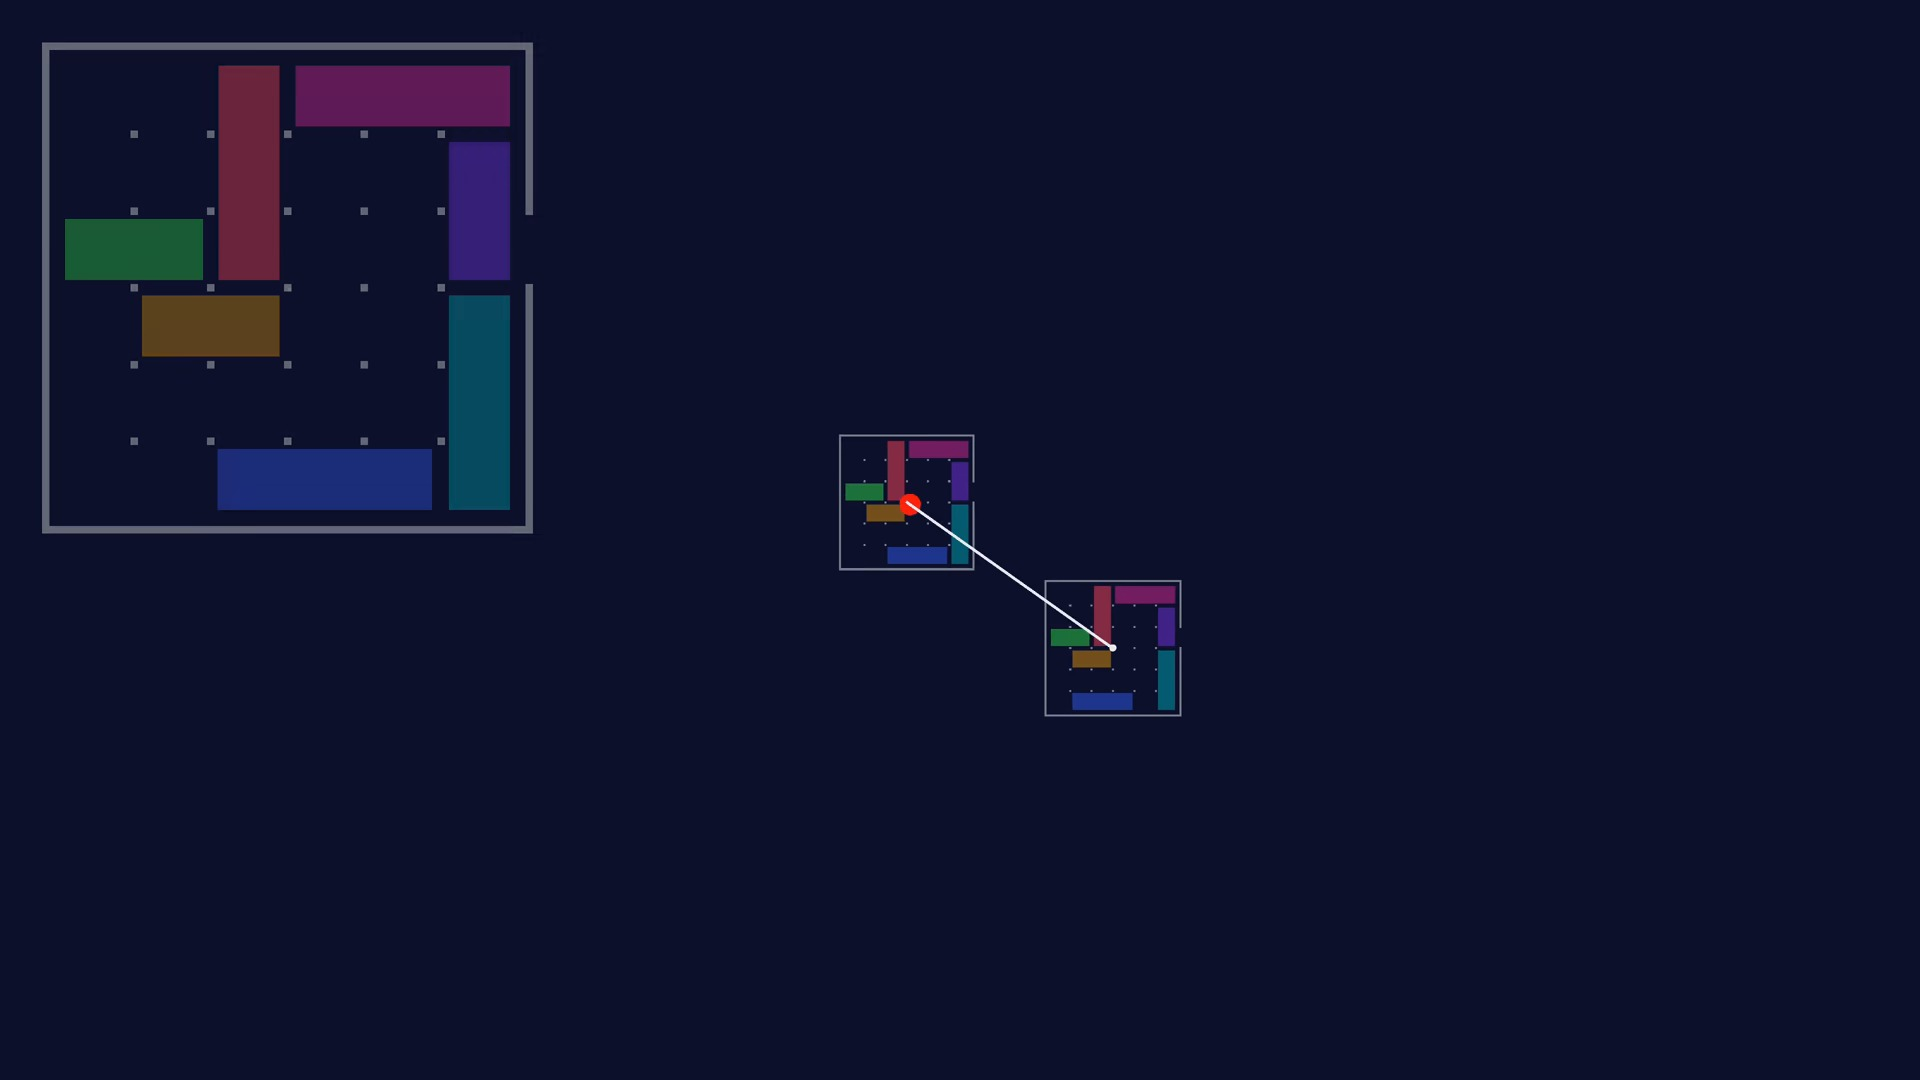
\includegraphics[width=0.90\textwidth]{figures/fig_02_nodes_and_edges.jpg}
\caption{左侧是当前 $6\times 6$ 盘面；右侧两张缩略图各代表一种局面，红点所在的节点与另一次滑动后的局面由一条边相连\vtag}
\end{figure}
\srcnote{00:00:38--00:00:54}
\end{minipage}

如果把\emph{全部}合法节点都画出来，这张图会是规整的格子，还是一团乱麻？要先建立直觉，讲者并不立刻处理华容道，而是从几道特意构造的、块与块几乎不相撞的小谜题讲起。

\subsection{本章小结}

盘面是节点，一次合法滑动是边。滑动积木因此不再只是桌上的玩具，而是一张同时具有局部子结构和全局超结构的状态图。接下来先看互不阻挡的积木，图会怎样长出来。

\section{互不阻挡时，每块积木就是一条运动轴}

先放进一块红色竖条。它只能沿着自己的轨道来回走，状态图因此是一条直线：只有一个自由度。

\noindent\begin{minipage}{\textwidth}
\begin{figure}[H]
\centering
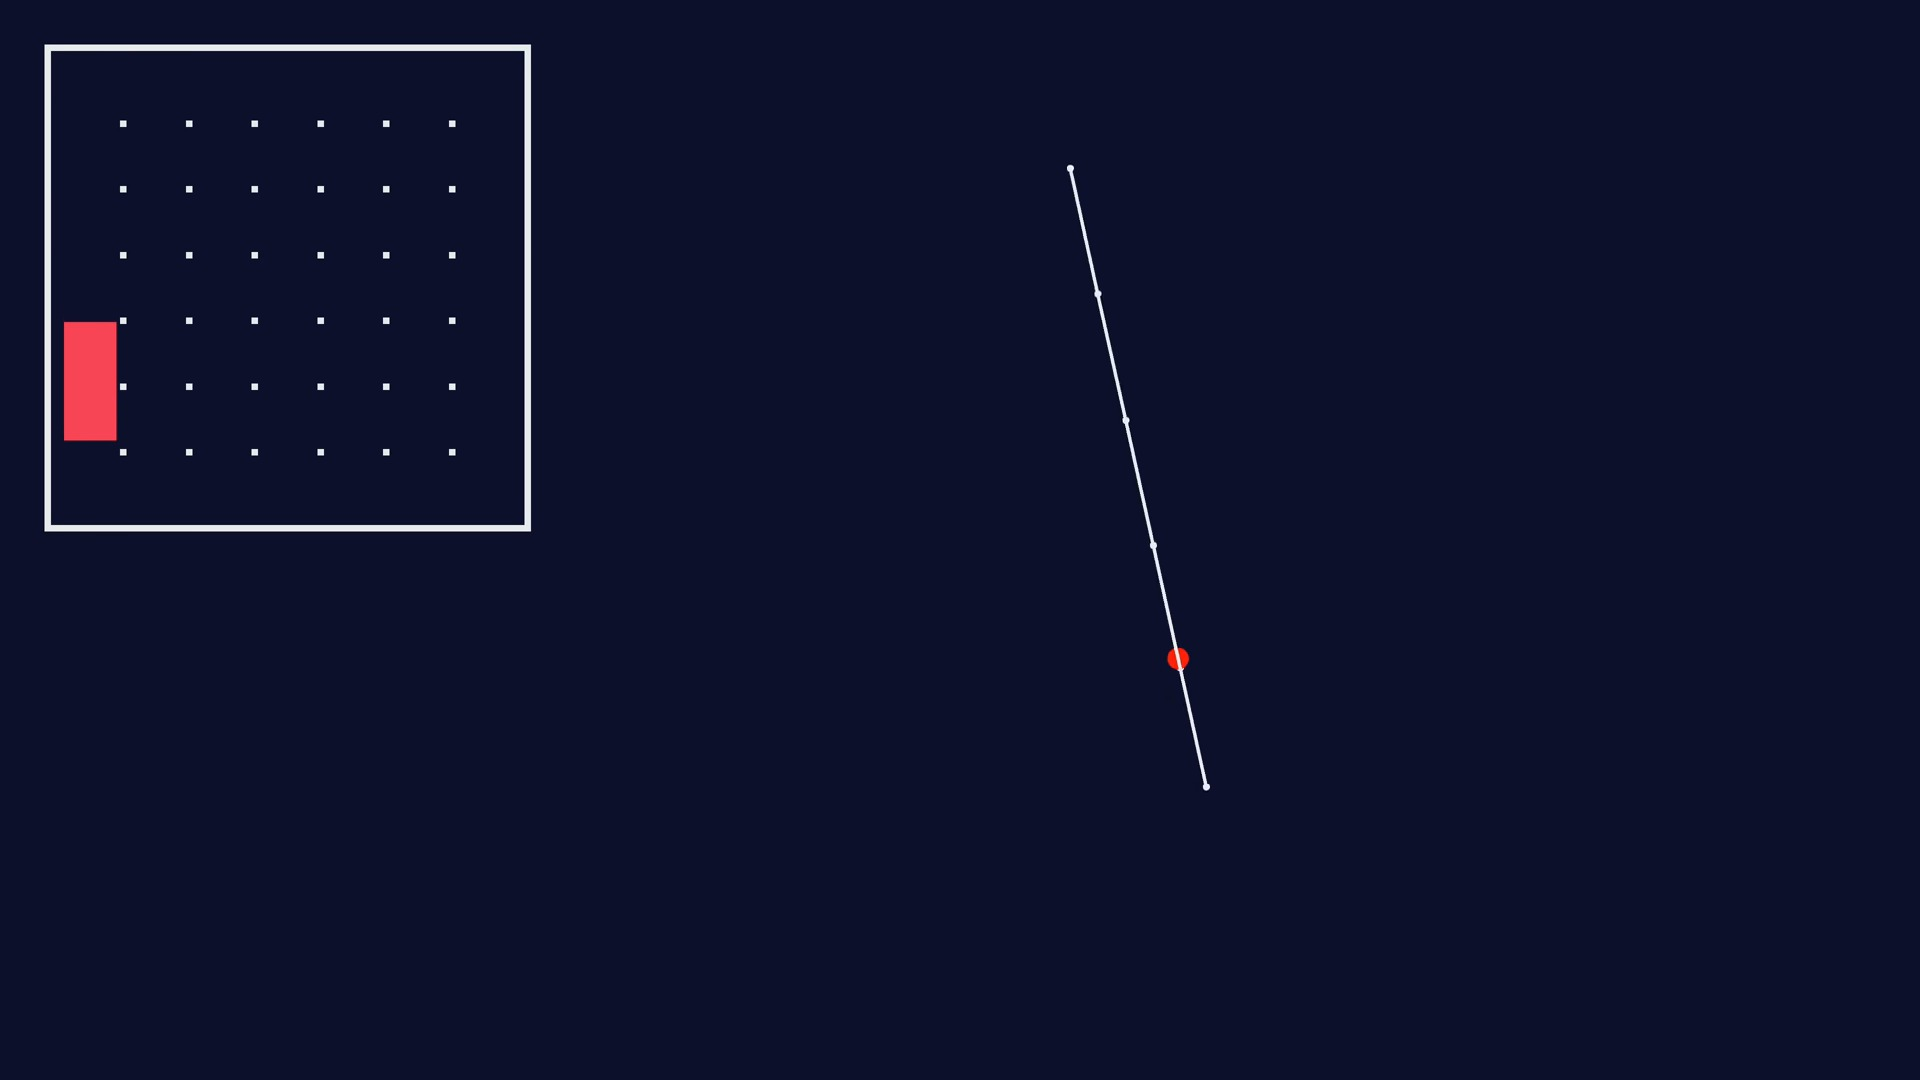
\includegraphics[width=0.90\textwidth]{figures/fig_03_one_block_line.jpg}
\caption{盘面上只有一块可滑动的红条，状态图退化成一条路径，红点标出当前坐标\vtag}
\end{figure}
\srcnote{00:01:18--00:01:22}
\end{minipage}

再并排放入第二块。两块都还能自由平移时，整体状态是两块各自坐标的笛卡尔积，于是得到一张二维网格。讲者的说法很干脆：每一块积木定义一条不同的运动轴。

\noindent\begin{minipage}{\textwidth}
\begin{figure}[H]
\centering
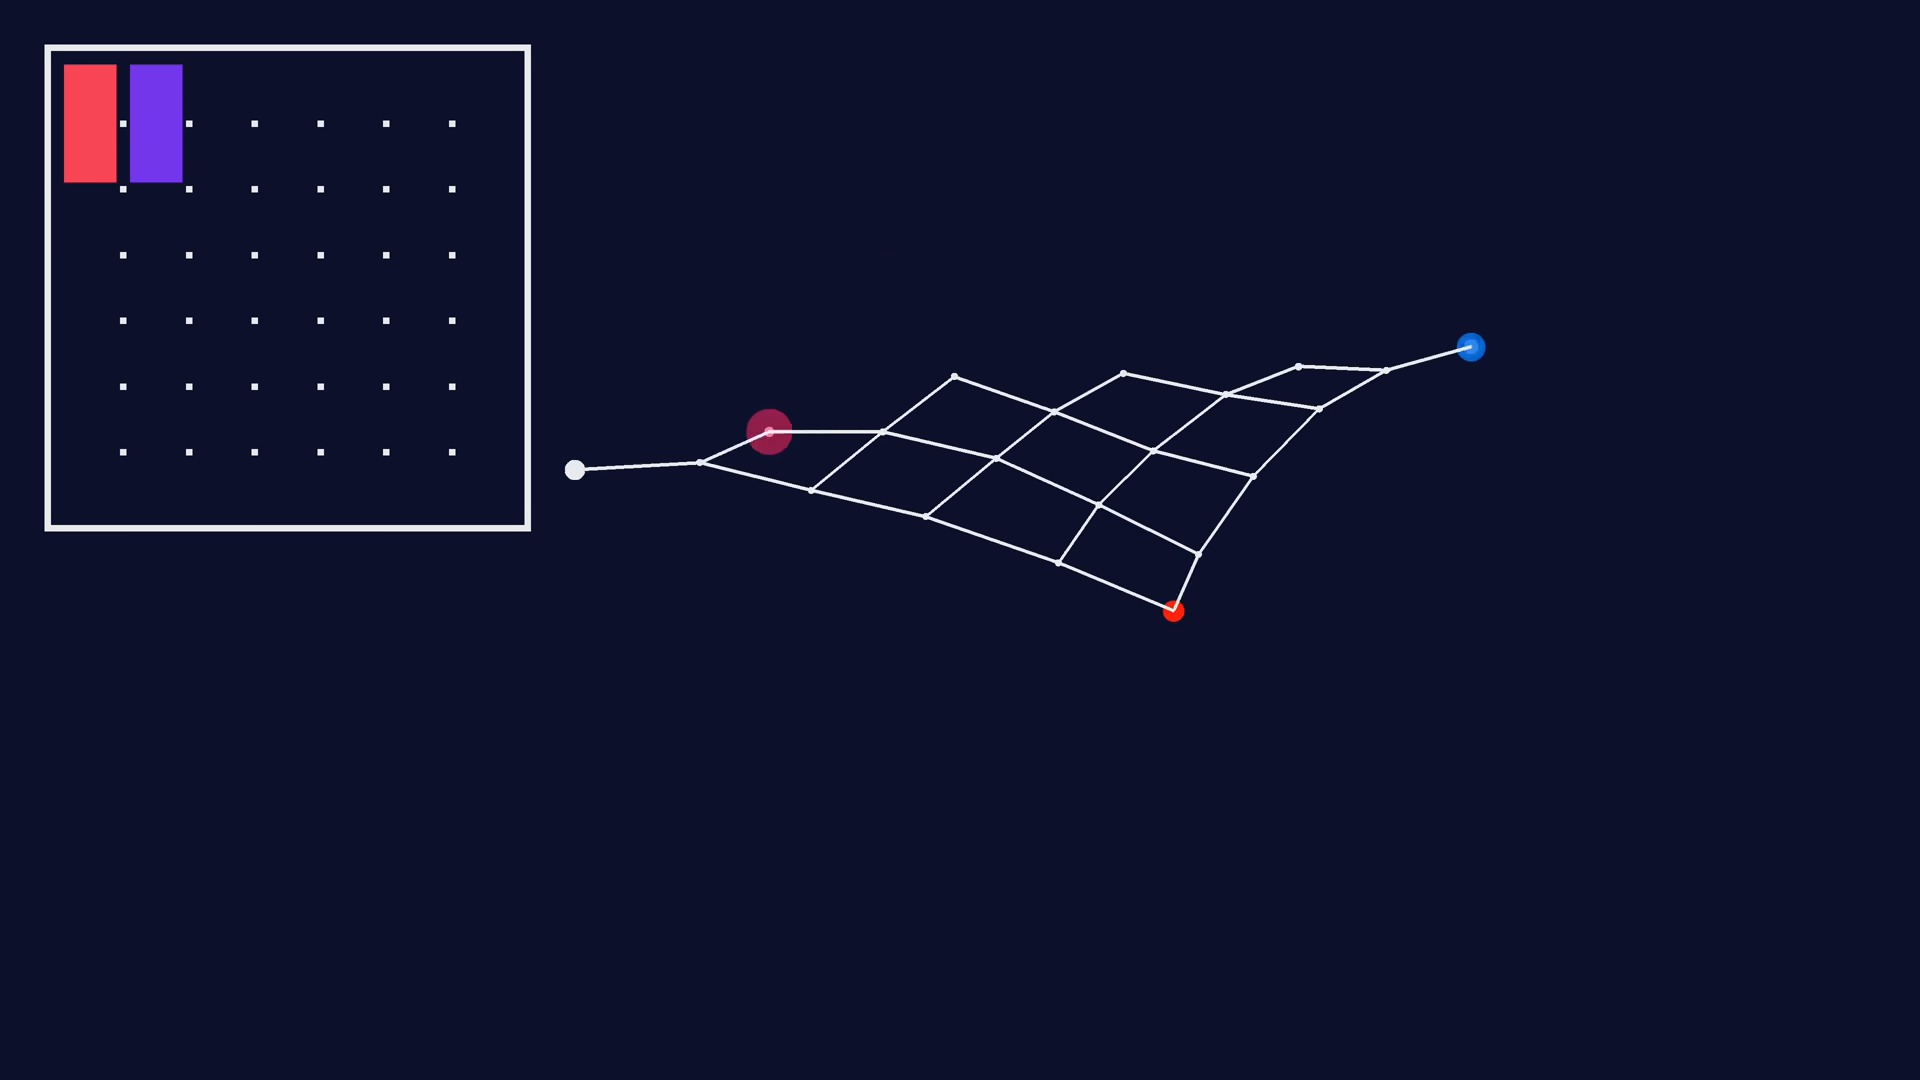
\includegraphics[width=0.90\textwidth]{figures/fig_04_two_block_grid.jpg}
\caption{红、紫两块互不阻挡时，状态图成为一张（略被投影压扁的）二维网格，各轴对应一块的坐标\vtag}
\end{figure}
\srcnote{00:01:22--00:01:27}
\end{minipage}

三块互不干涉，图就长成三维格子；自由度再加到四个，图会自然伸展成超立方体那样的高维骨架。这些构造谜题的意义在于先给出一个干净的参照：在没有碰撞的世界里，图的维数几乎就等于块的个数。

\noindent\begin{minipage}{\textwidth}
\begin{figure}[H]
\centering
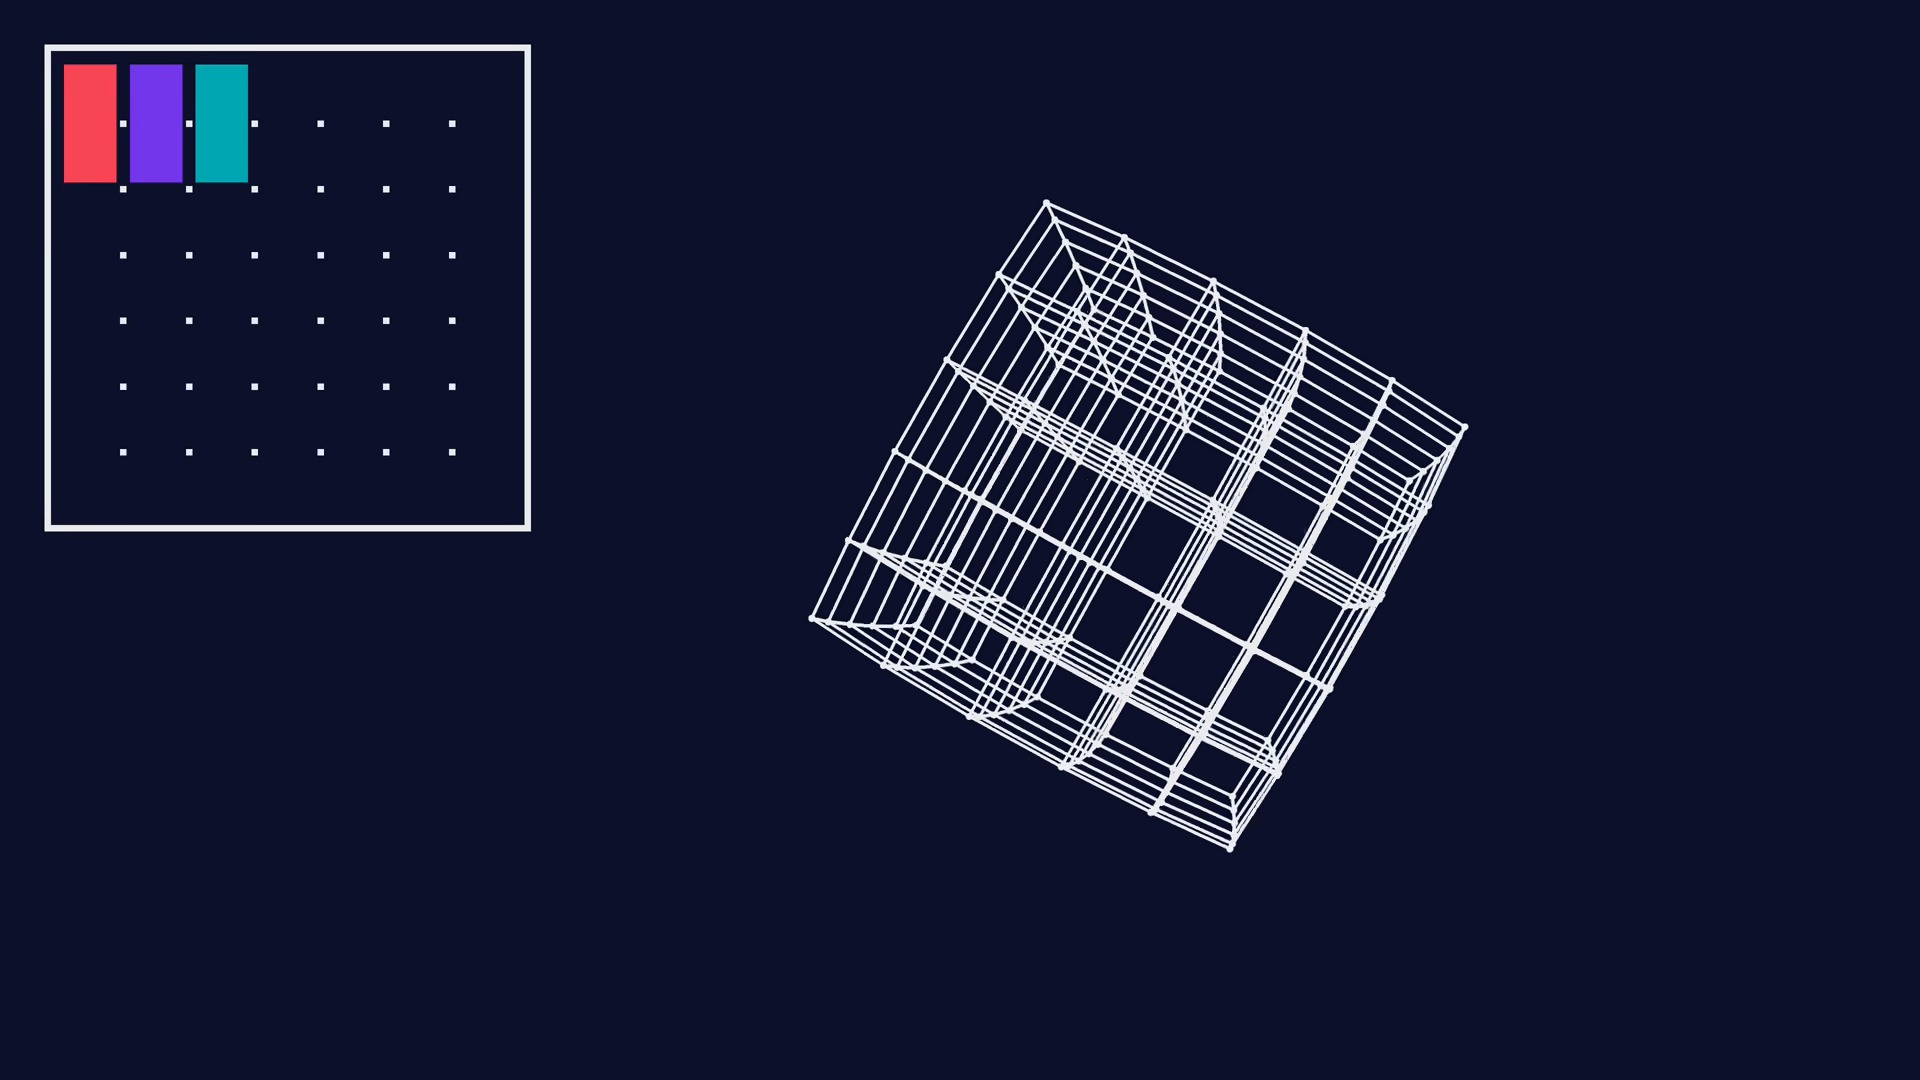
\includegraphics[width=0.90\textwidth]{figures/fig_05_three_block_lattice.jpg}
\caption{三块平行竖条对应一张三维格子，节点沿三条互相独立的运动轴排列\vtag}
\end{figure}
\srcnote{00:01:34--00:01:38}
\end{minipage}

\noindent\begin{minipage}{\textwidth}
\begin{figure}[H]
\centering
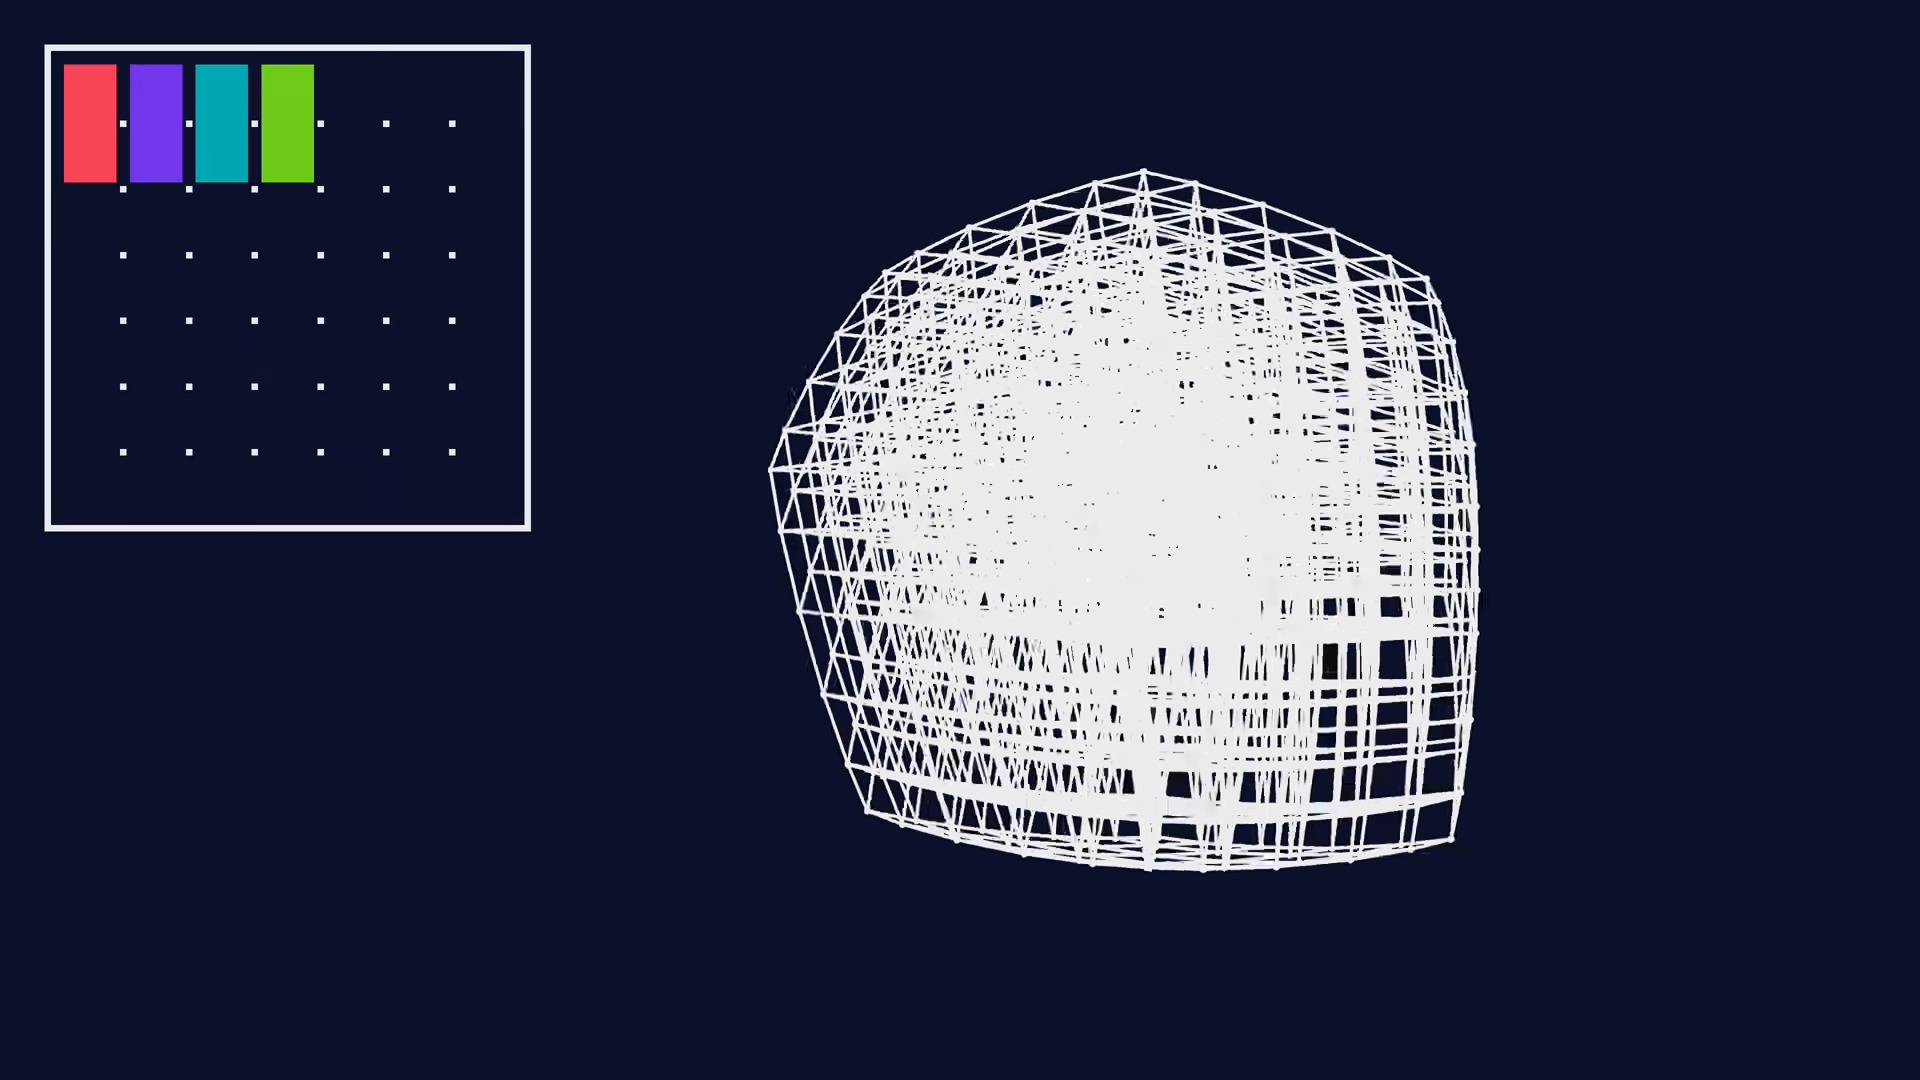
\includegraphics[width=0.90\textwidth]{figures/fig_06_four_dof_hypercube.jpg}
\caption{四个自由度时，状态图进一步填满超立方体式的高维网格\vtag}
\end{figure}
\srcnote{00:01:38--00:01:43}
\end{minipage}

\subsection{本章小结}

在块与块可以彼此穿过、互不占位的理想情形下，每块积木是一条坐标轴，两块给出网格，三块给出三维格子，四个自由度则伸向超立方体。真正有趣的变化，发生在它们开始互相挡住的时候。

\section{一旦积木会相撞，合法状态就会被挖空}

把刚才那道两块谜题改成两块相向而立，二维网格就不再完整：有一块区域从结构里消失了，那里对应两块在几何上重叠的非法局面。剩下的图看起来像被挖掉中心的环廊。

\noindent\begin{minipage}{\textwidth}
\begin{figure}[H]
\centering
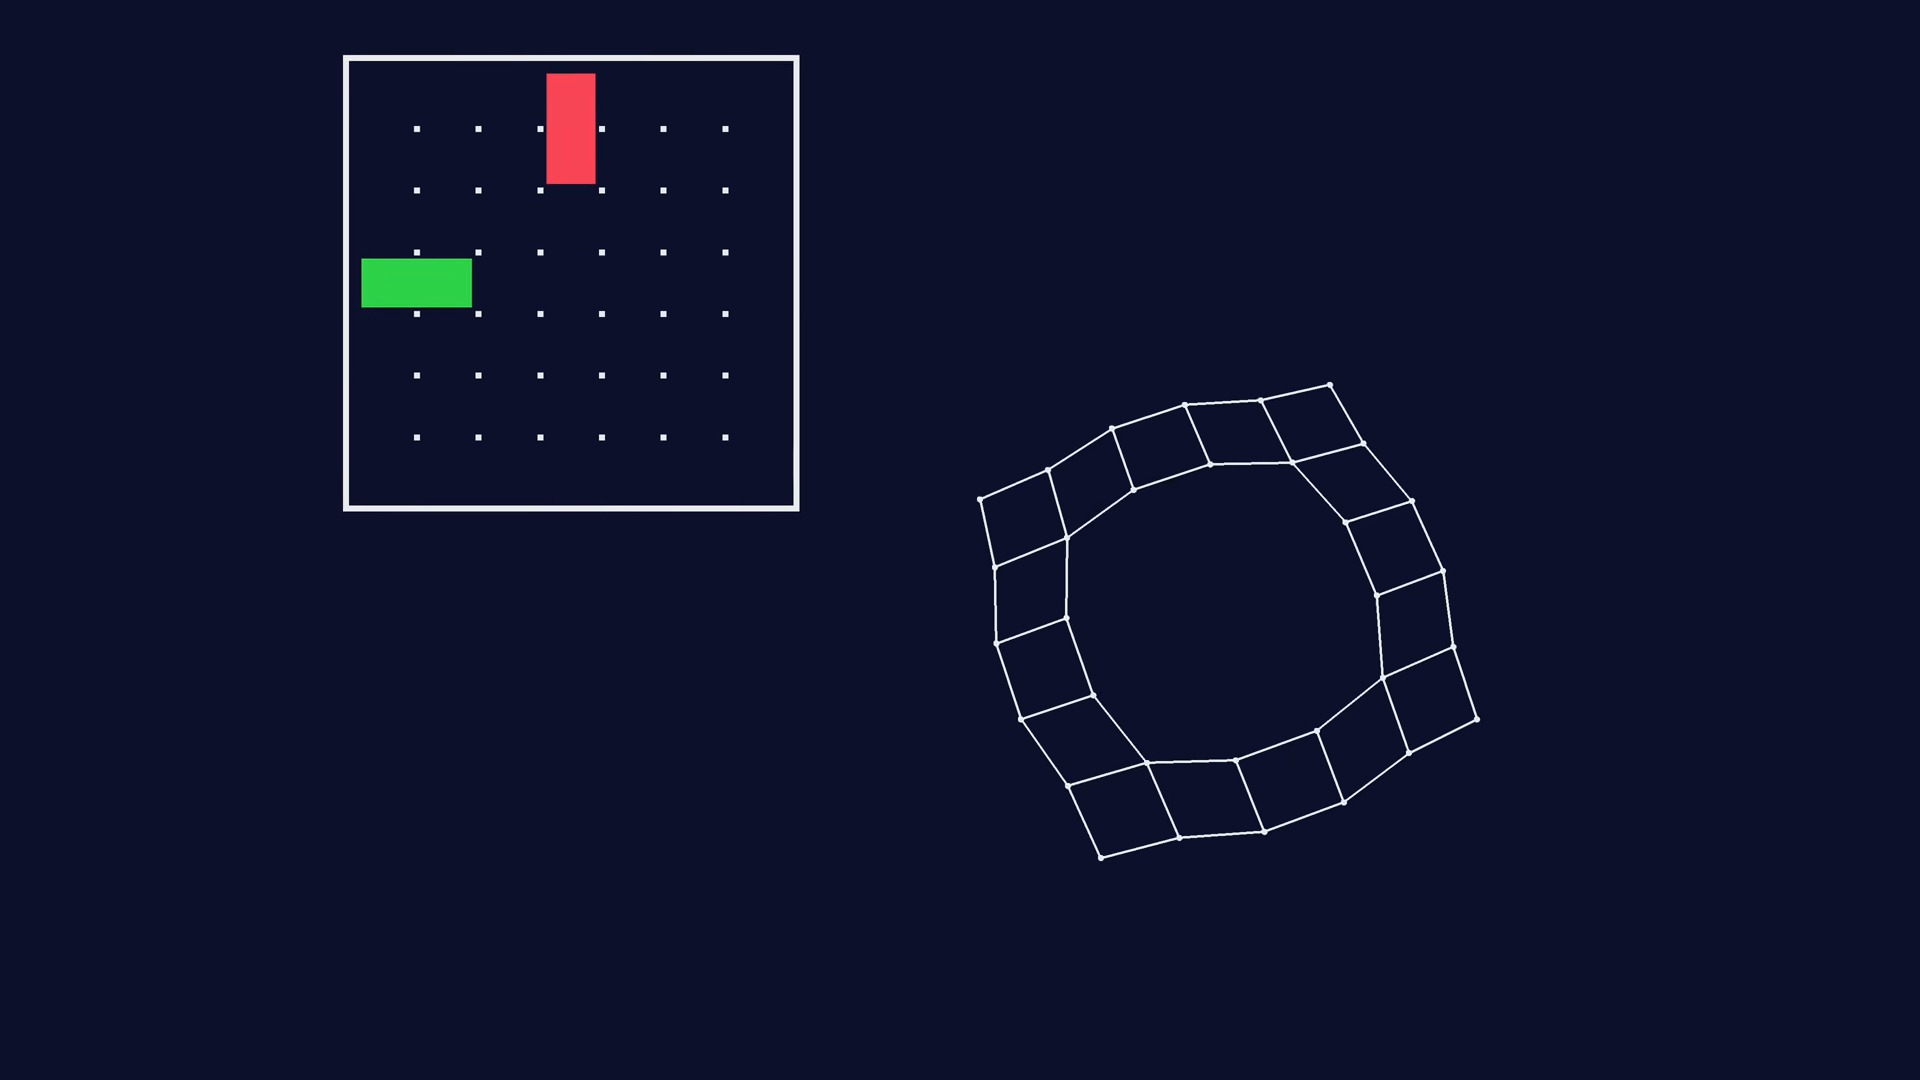
\includegraphics[width=0.90\textwidth]{figures/fig_07_opposing_invalid.jpg}
\caption{红竖条与绿横条相向布置时，表示两块重叠的那部分二维结构不再合法，图中央出现空洞\vtag}
\end{figure}
\srcnote{00:01:47--00:02:08}
\end{minipage}

若两块被放进同一条轨道，一前一后，图形会变成三角形：不论前方那块滑到哪里，它都构成后方那块的边界。后方不能穿过前方，可到达的坐标对便被裁成一块直角区域。

\noindent\begin{minipage}{\textwidth}
\begin{figure}[H]
\centering
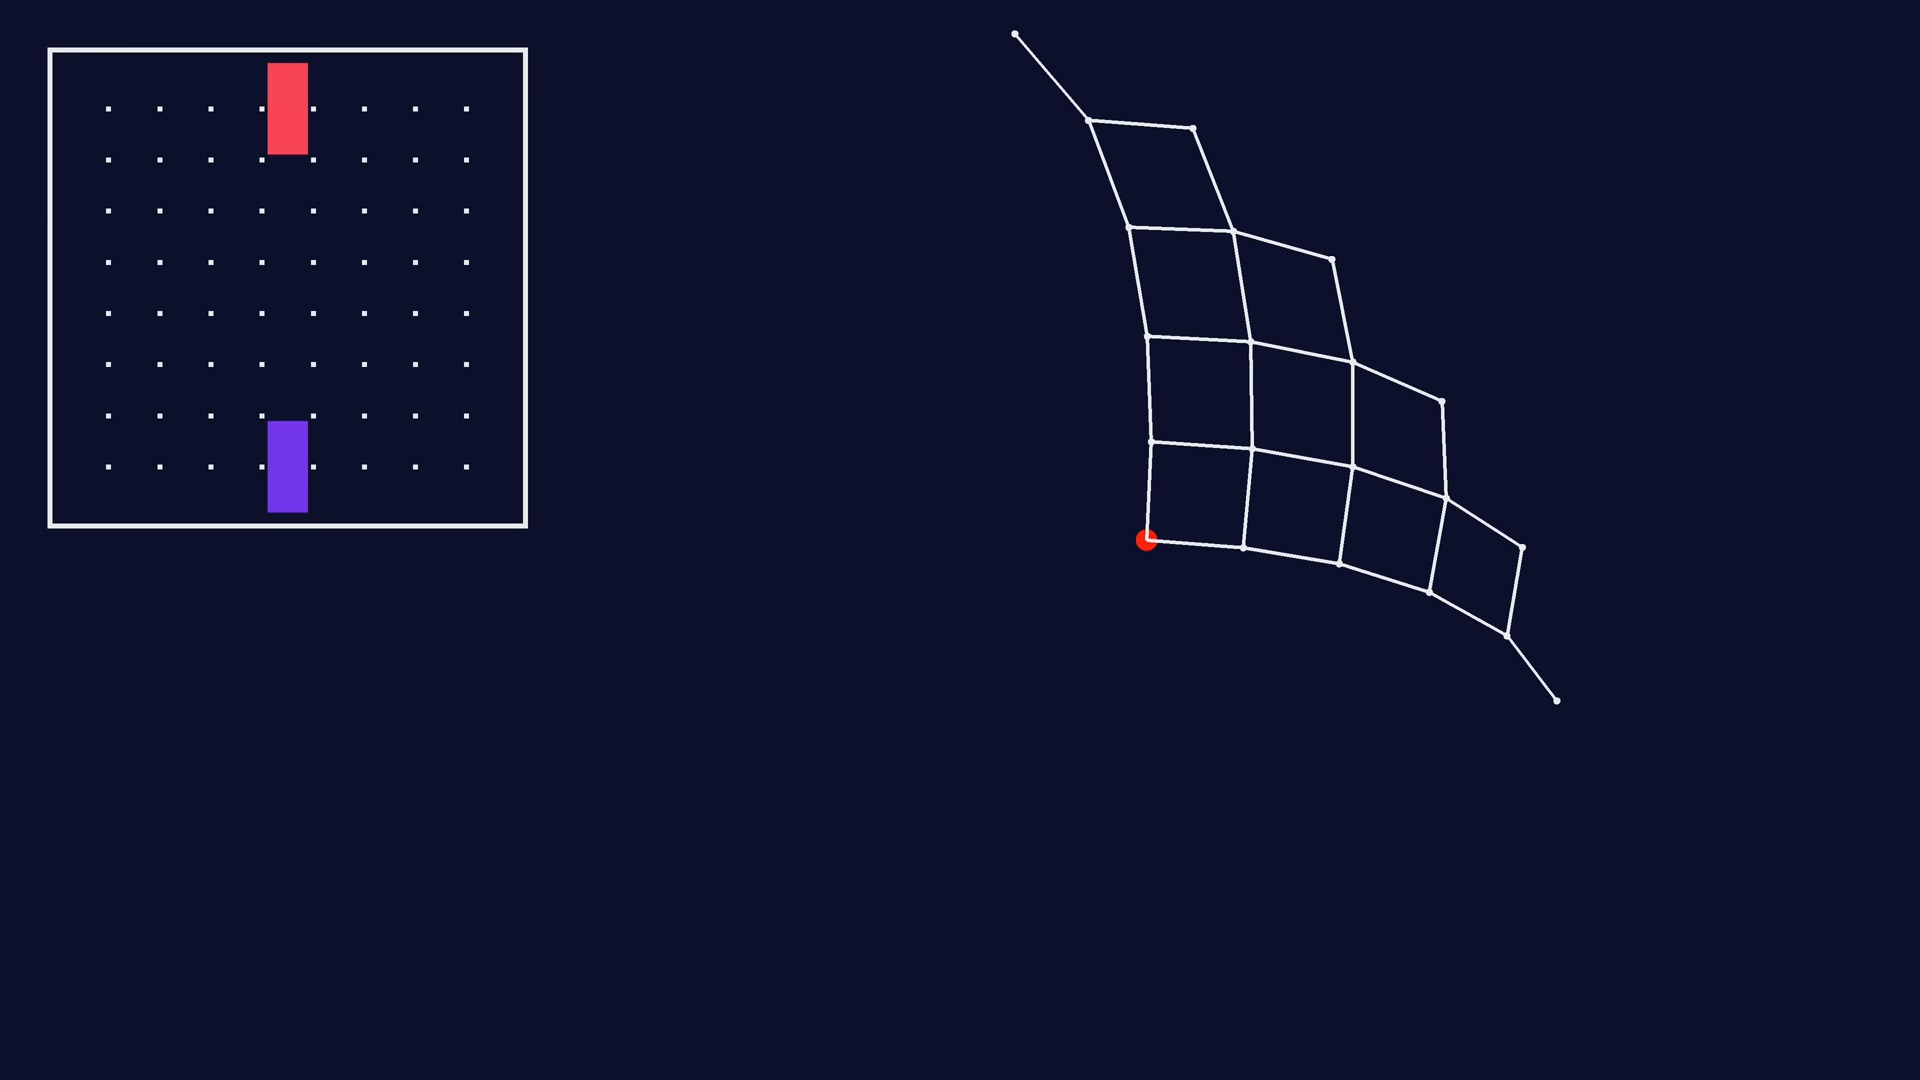
\includegraphics[width=0.90\textwidth]{figures/fig_08_same_lane_triangle.jpg}
\caption{同一列上的红、紫两块一前一后，状态图呈三角形：上方块的位置为下方块设下上界\vtag}
\end{figure}
\srcnote{00:02:08--00:02:20}
\end{minipage}

这类谜题还悄悄制造了一个“想象中的对偶结构”。把两块对调之后，许多盘面在几何上仍然合法，却无法在不让一块穿过另一块的前提下到达。于是图上会出现与可达三角形隔开的另一块三角形：形状对称，却不属于当前连通的世界。

\noindent\begin{minipage}{\textwidth}
\begin{figure}[H]
\centering
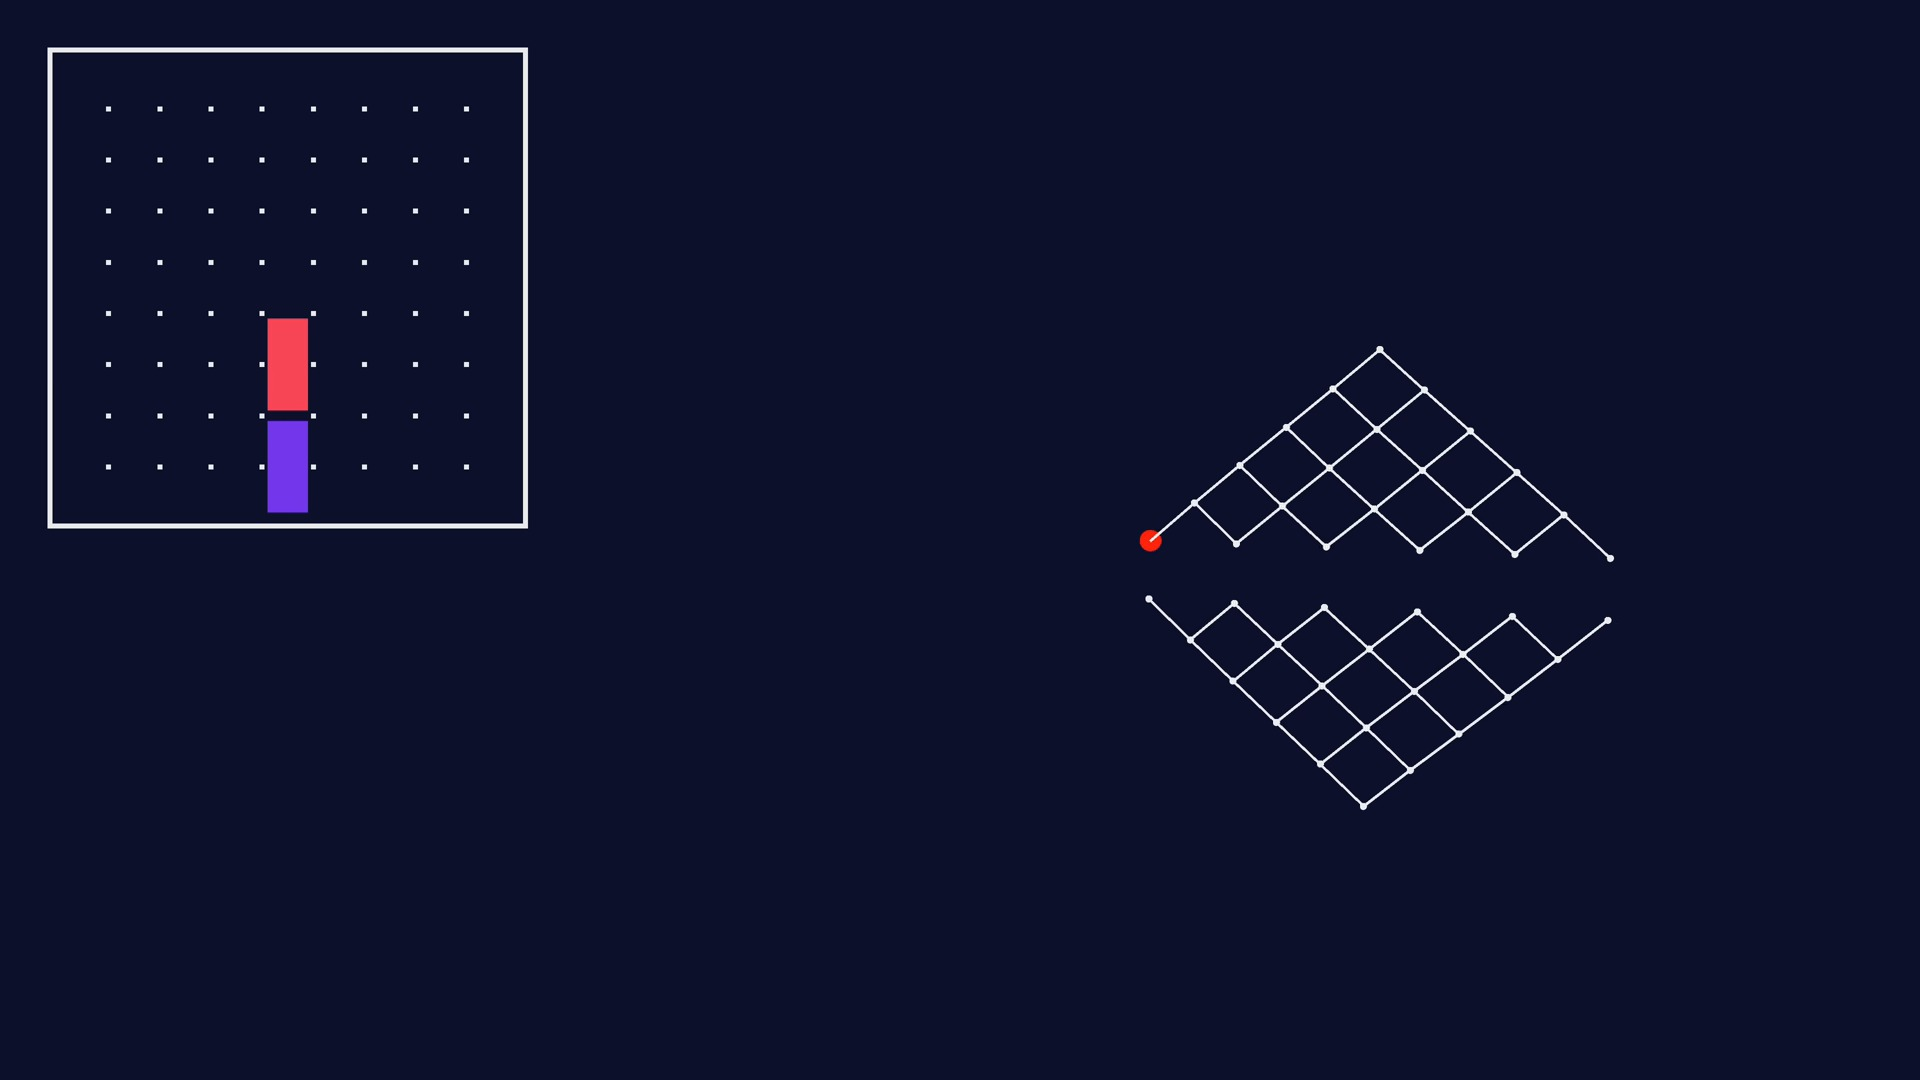
\includegraphics[width=0.90\textwidth]{figures/fig_09_imaginary_counterpart.jpg}
\caption{上方带红点的三角形是当前可达分量；下方那块对偶三角形对应必须穿块才能进入的合法局面\vtag}
\end{figure}
\srcnote{00:02:20--00:02:33}
\end{minipage}

三块互相干涉时，主体仍可看成立方体，只是一些区域被挖空。块数再升高，图的维数就越来越不像“有几块就有几维”，而更取决于有多少空位。

\subsection{本章小结}

碰撞会从理想网格里删去重叠状态，同一轨道会把矩形裁成三角形，还会分出“合法但不可达”的对偶分量。维数的主导因素，开始从块数转向空位。

\section{空位才是自由度：局部的二维流形}

讲者接着展示一道块数更多的谜题，并把整张状态图完全展开。整体上能看出一种超结构，但截取一小段来看，局部又排列得相当整齐，像一块二维的欧氏流形，恰好有两个自由度。原因就在盘面上：有两个可以让积木滑动的空洞。一个轴对应推动上方的空洞，另一个轴对应推动下方的空洞。

\noindent\begin{minipage}{\textwidth}
\begin{figure}[H]
\centering
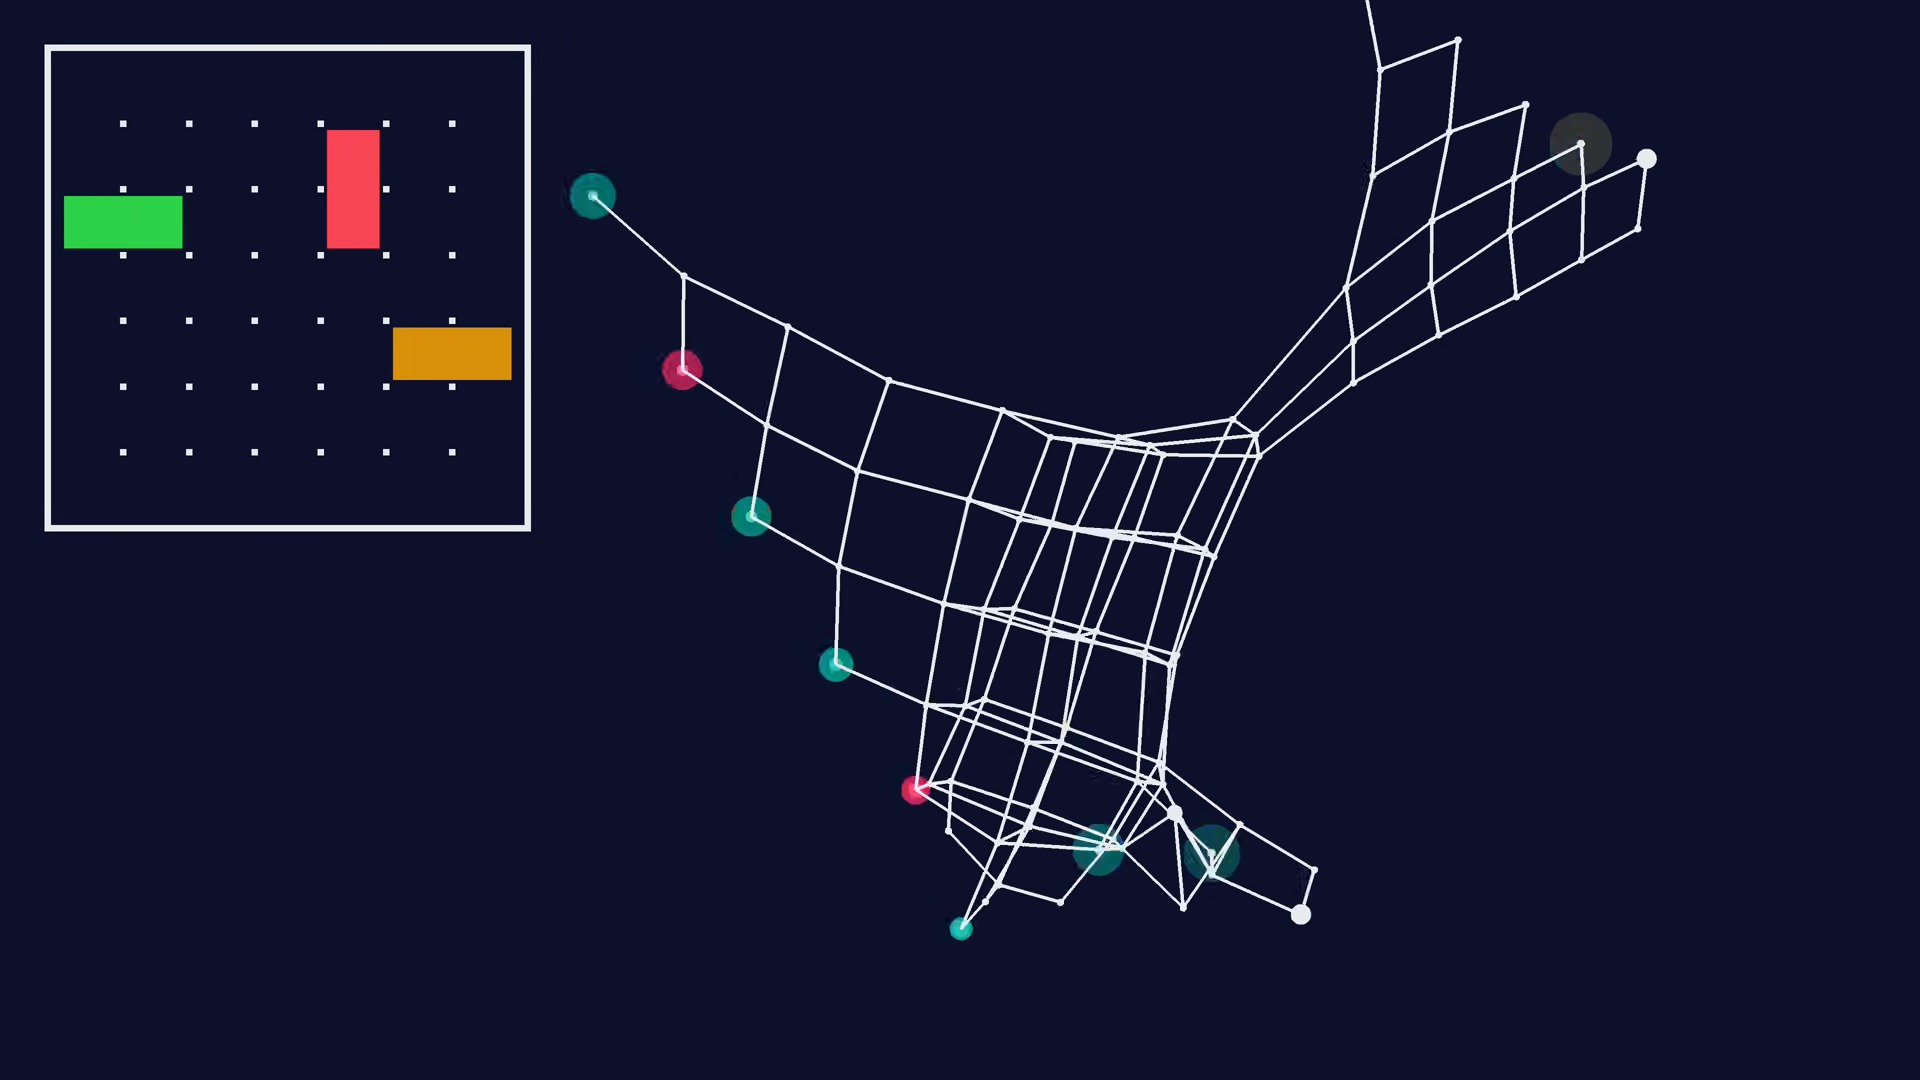
\includegraphics[width=0.90\textwidth]{figures/fig_10_local_superstructure.jpg}
\caption{把更拥挤的一盘完全展开后，图既有整体的超结构，也在局部出现规则的网格状区域\vtag}
\end{figure}
\srcnote{00:02:49--00:03:05}
\end{minipage}

\noindent\begin{minipage}{\textwidth}
\begin{figure}[H]
\centering
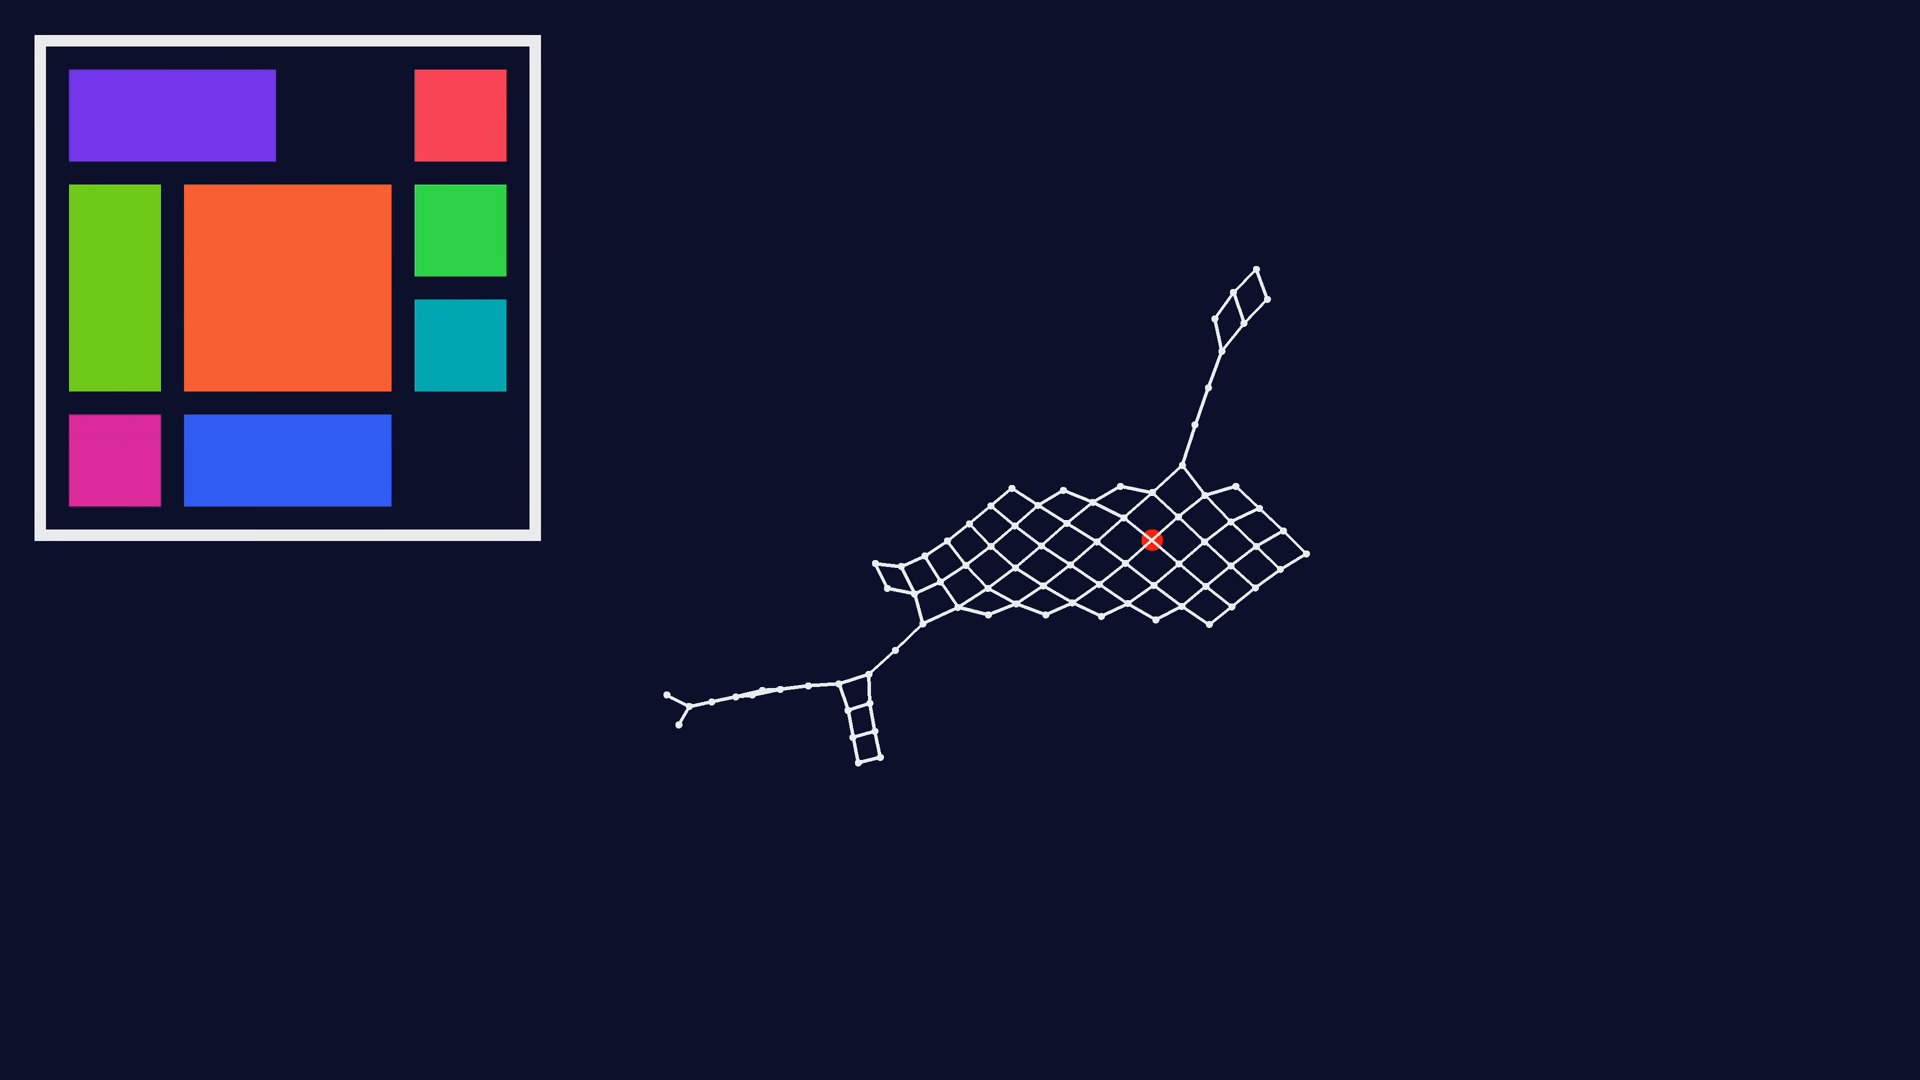
\includegraphics[width=0.90\textwidth]{figures/fig_11_local_manifold.jpg}
\caption{盘面上两个空洞对应局部二维流形：中间那片菱形网格，正是两空位各自平移所张成的平面\vtag}
\end{figure}
\srcnote{00:03:05--00:03:23}
\end{minipage}

讲者把这句话推到极限：在极端情形下，并不是积木在动，而是空位在定义自由度。棋盘完全填满时几乎动不了，完全空旷时又只剩下若干独立的平移；介于两者之间，才会出现块与块缠绕、交切而成的复杂结构。

若把两个空位的坐标记为 $(h_1,h_2)$，那么在它们尚未被别的块锁死的那一段里，局部状态就可以看成
\[
(h_1,h_2)\in\mathbb{Z}^2,
\]
每个空位提供一条独立的运动轴。这不是讲者写在黑板上的公式，而是他把“两个空洞、两个自由度”说成局部欧氏流形时，盘面坐标本身的记法。

\subsection{本章小结}

块很多时，真正决定局部维数的是空位。两个空洞会在图上长出一块二维网格；整张图则是这种局部规则与全局缠绕叠在一起的结果。

\begin{importantbox}{空位比块数更决定局部维数}
讲者在块数升高之后反复强调：这时图的维数与积木块数的关系变弱，更主要取决于还能推动的空位。两个空洞就会在局部长出一块二维欧氏流形。也可以更极端地说，并不是积木在动，而是空位在定义可以走的方向。
\end{importantbox}

\section{红杠谜题：四个角上的正方形超结构}

讲者回到开场用过的那道 $6\times 6$ 出口谜题，请观众先猜它的超结构。从稍稍倾斜的视角看，盘面几乎是对称的。关键在于两块水平积木（绿与橙）会分别卡在竖直红杠的左侧或右侧，而且同一时刻只有一块能越过这根杠。红杠抬起时，橙块可以过渡到另一侧；红杠落下时，则轮到绿块过渡。

\noindent\begin{minipage}{\textwidth}
\begin{figure}[H]
\centering
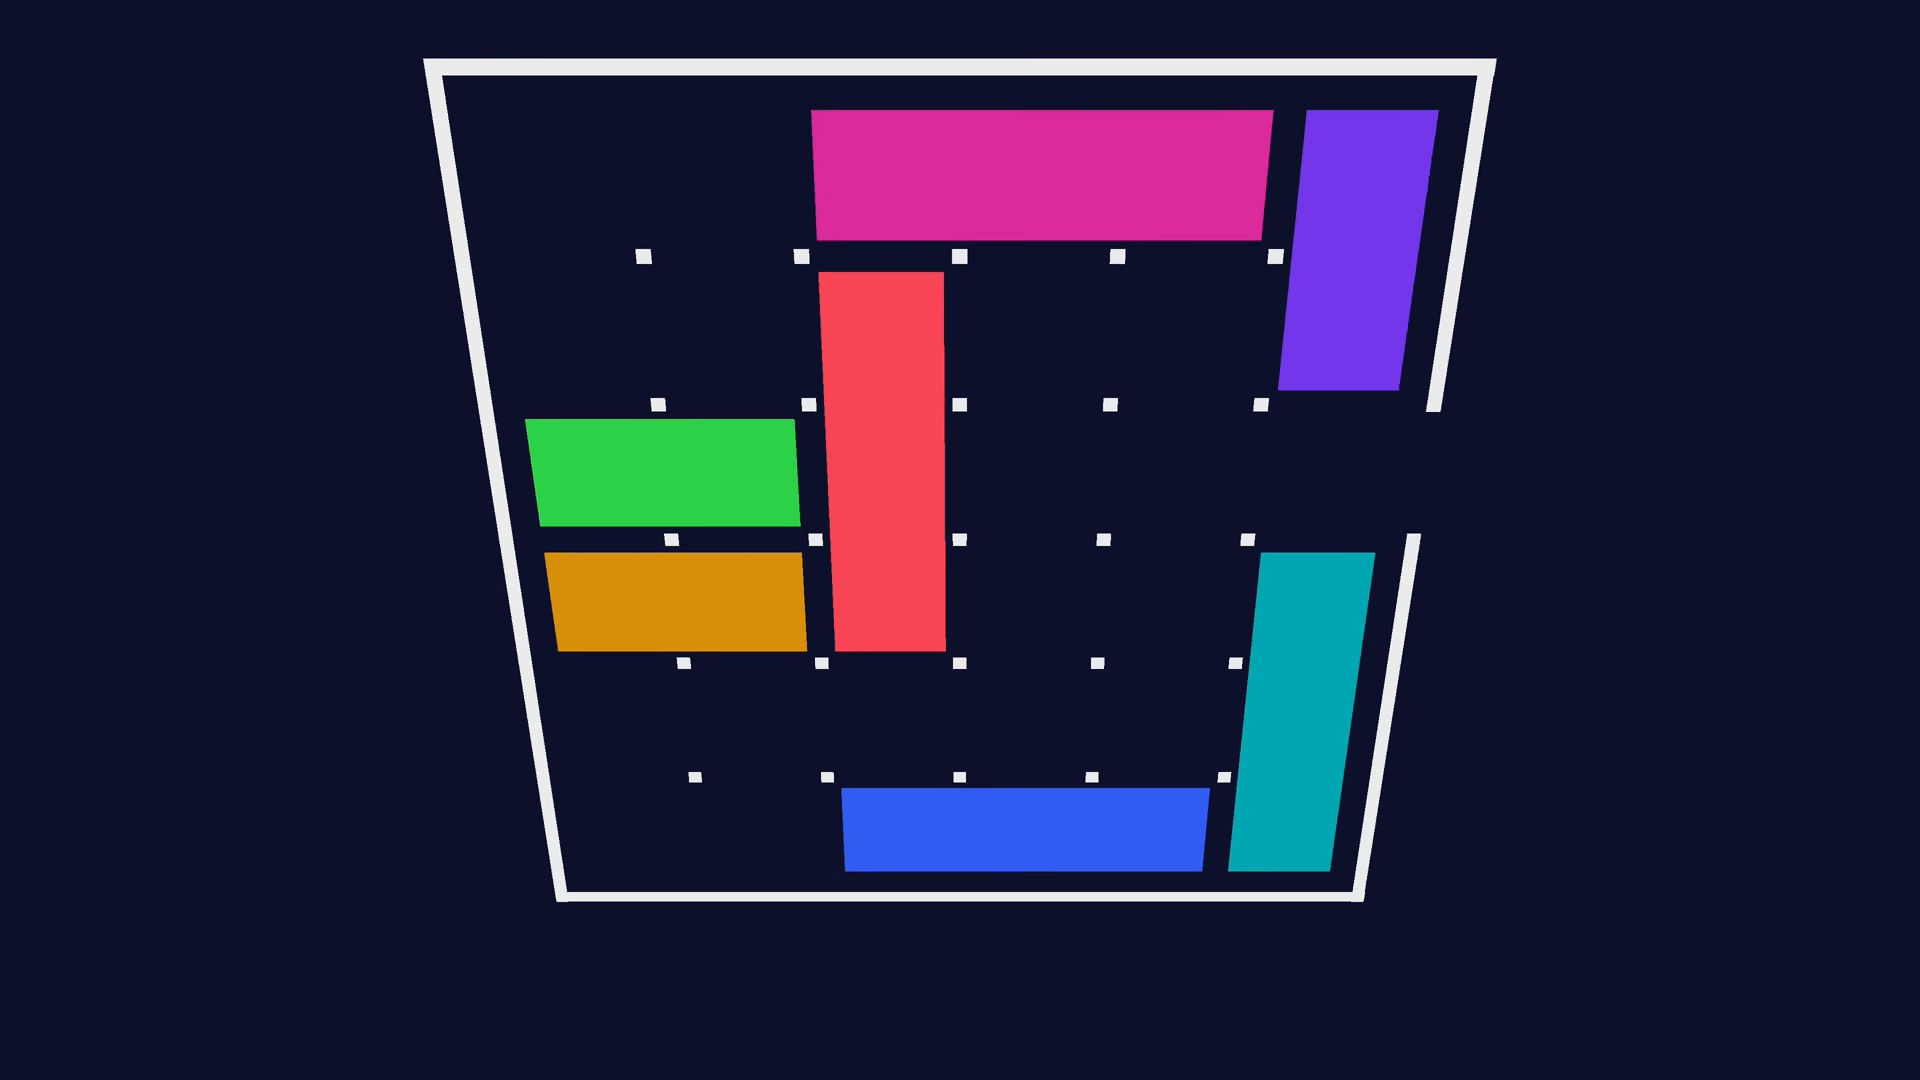
\includegraphics[width=0.90\textwidth]{figures/fig_12_redbar_puzzle.jpg}
\caption{开场那道 $6\times 6$ 谜题：右侧有出口，竖直红杠把绿、橙两块隔在不同的“卡位”里\vtag}
\end{figure}
\srcnote{00:03:38--00:03:57}
\end{minipage}

\noindent\begin{minipage}{\textwidth}
\begin{figure}[H]
\centering
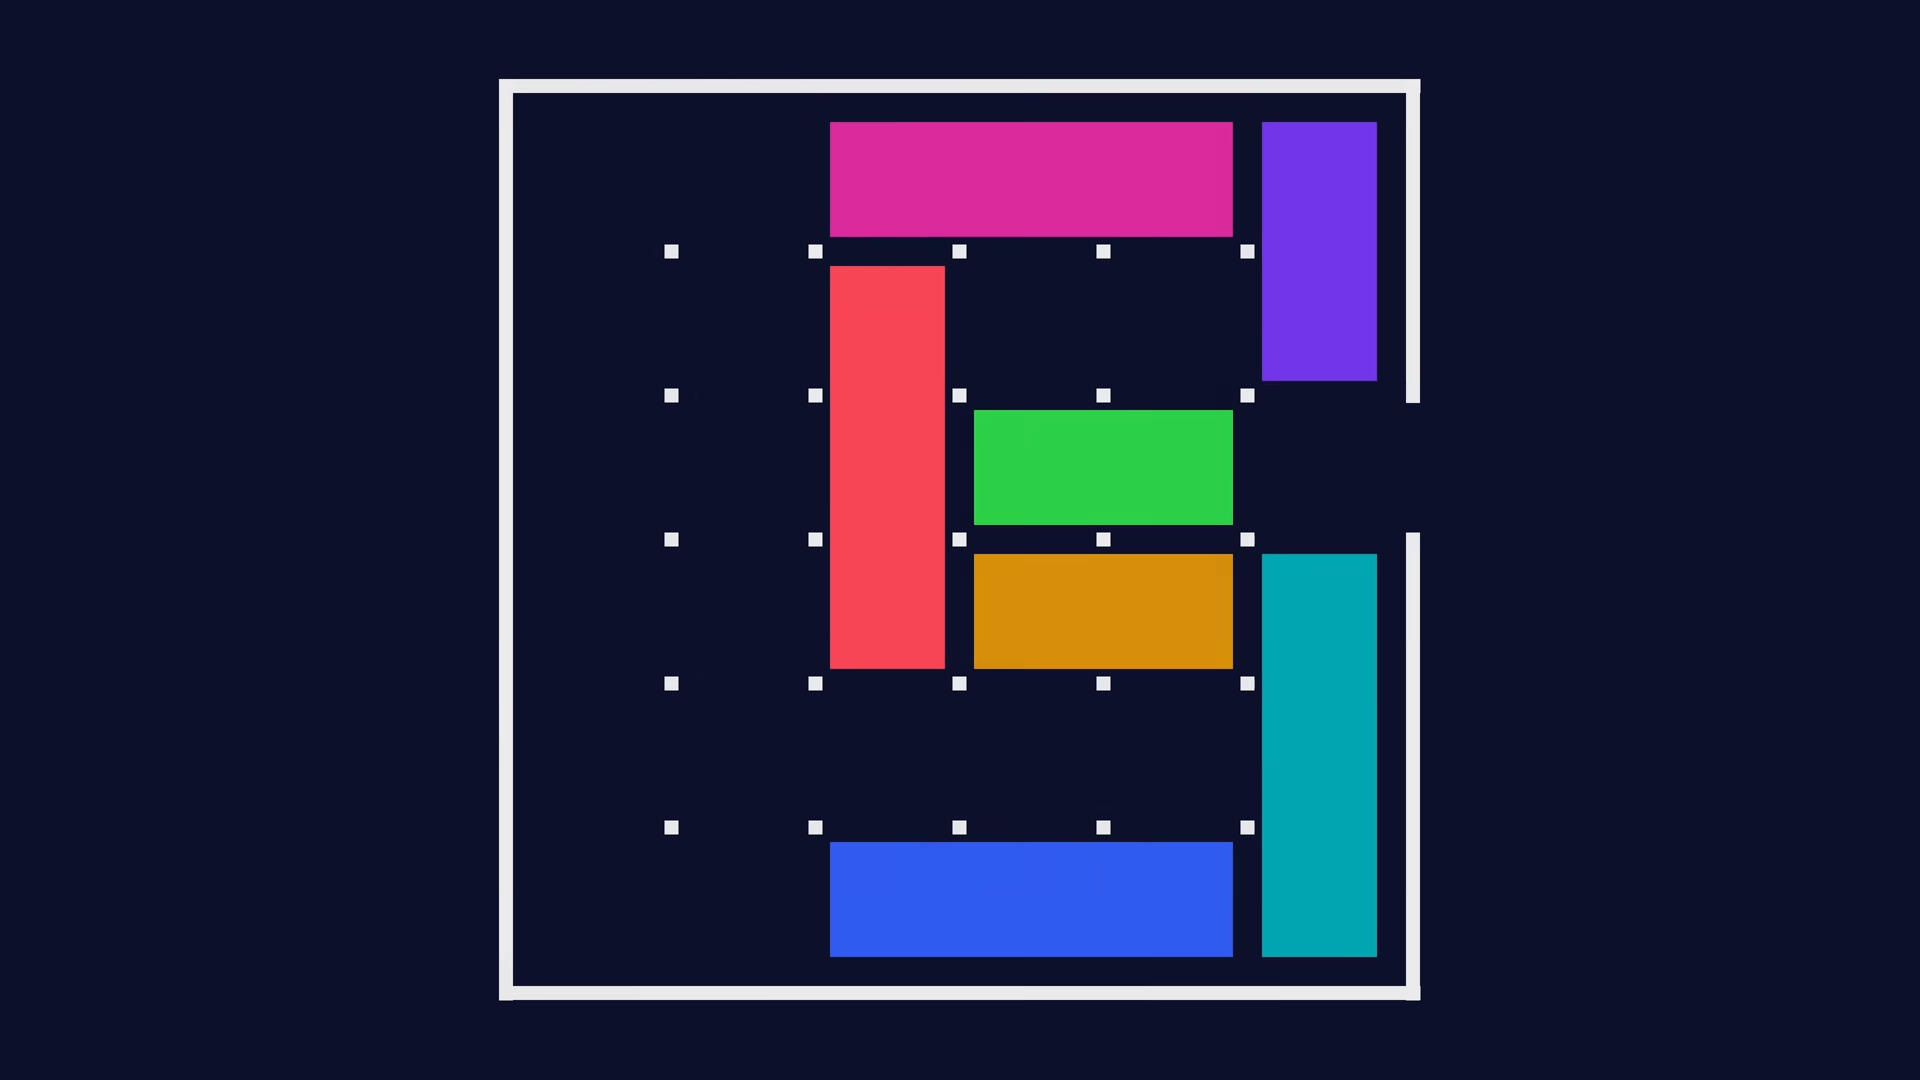
\includegraphics[width=0.90\textwidth]{figures/fig_13_latch_left_right.jpg}
\caption{绿块与橙块都已翻到竖直红杠的右侧；它们各自只能处于杠左或杠右两种卡位之一\vtag}
\end{figure}
\srcnote{00:03:57--00:04:11}
\end{minipage}

把全部节点按其盘面着色，超结构就显现出来：它是一个连接四个角的正方形。四个角附近节点特别密，维数明显高于四条边。一半节点对应“绿块已在红杠右侧”，另一半对应“橙块已在红杠右侧”。解——绿块贴在右侧出口——毫不意外地全部落在绿块已经翻到右侧的那些角上。至于角上为什么维数更高，讲者把这个问题留给观众，随即把话题转向华容道本身。

\noindent\begin{minipage}{\textwidth}
\begin{figure}[H]
\centering
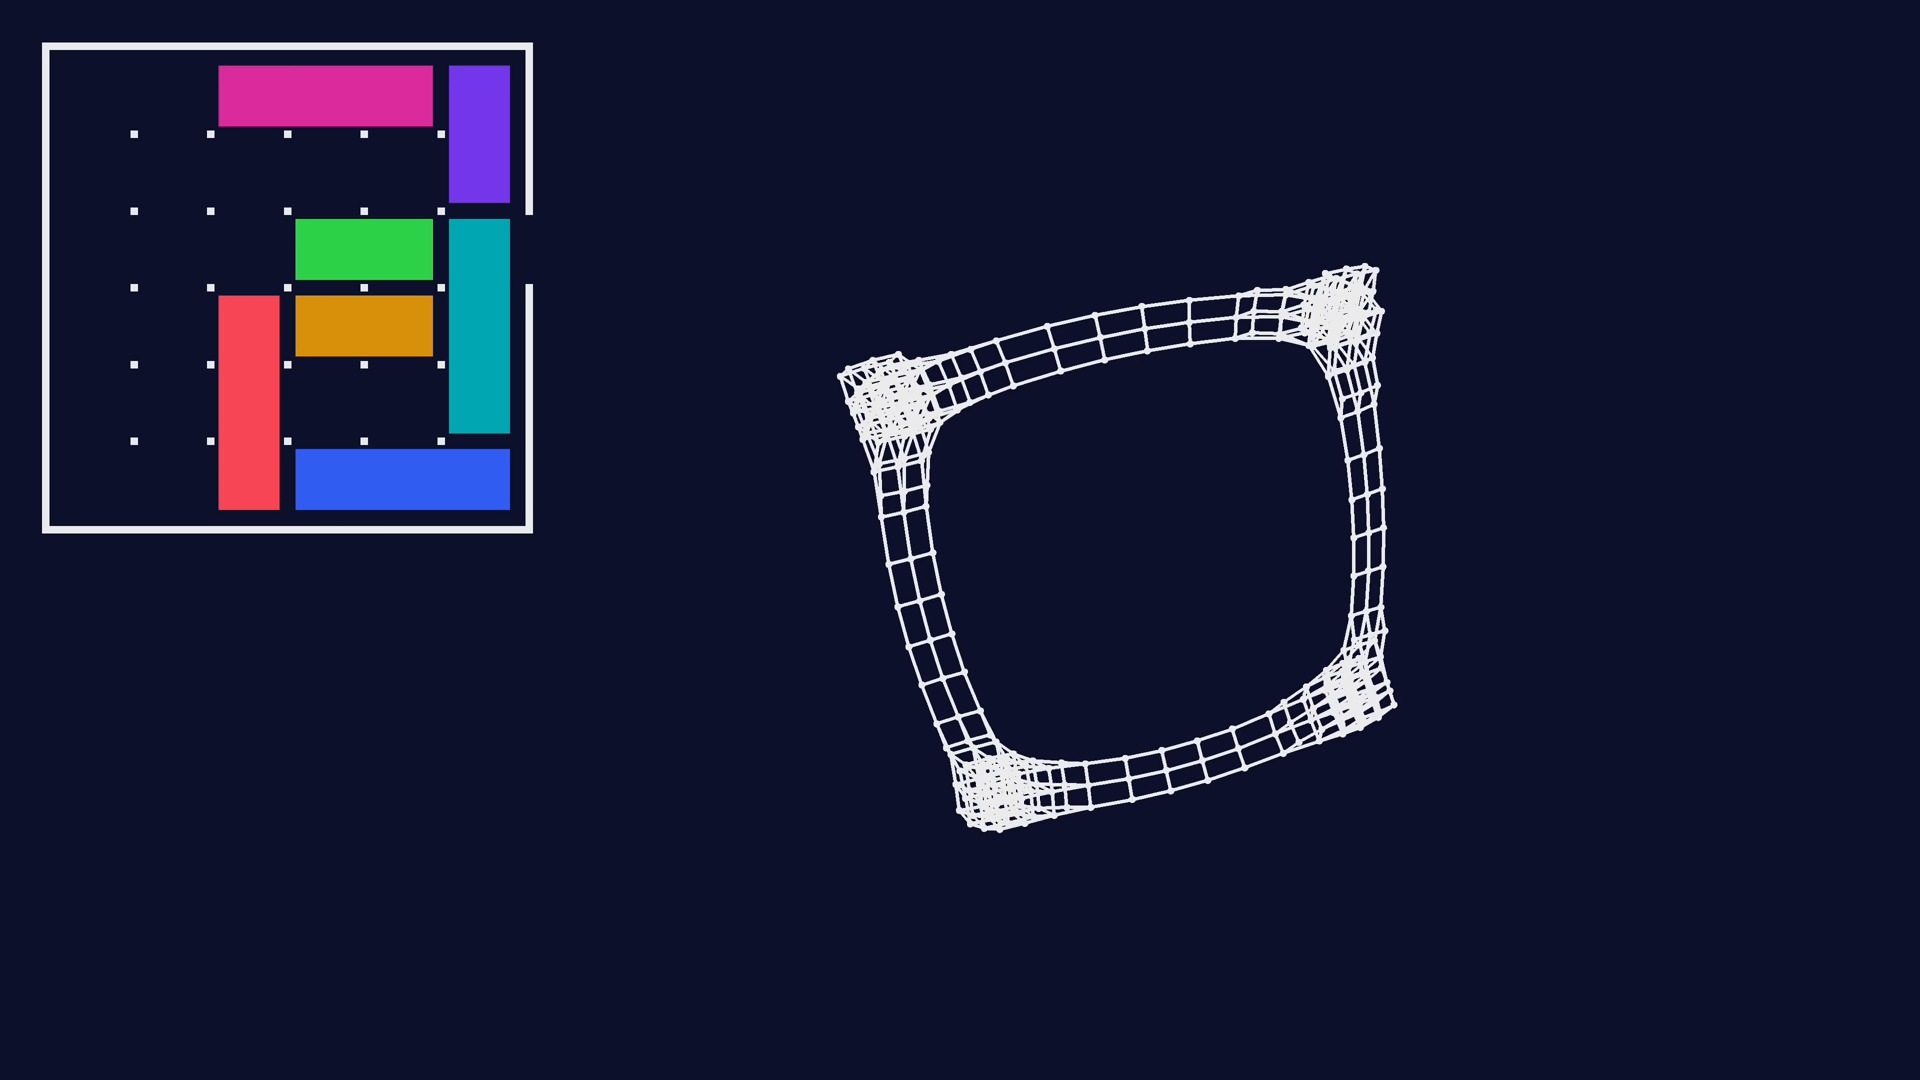
\includegraphics[width=0.90\textwidth]{figures/fig_14_square_four_corners.jpg}
\caption{这道谜题的超结构是连接四个角的正方形，角上网格更密，边则相对细瘦\vtag}
\end{figure}
\srcnote{00:04:21--00:04:32}
\end{minipage}

\noindent\begin{minipage}{\textwidth}
\begin{figure}[H]
\centering
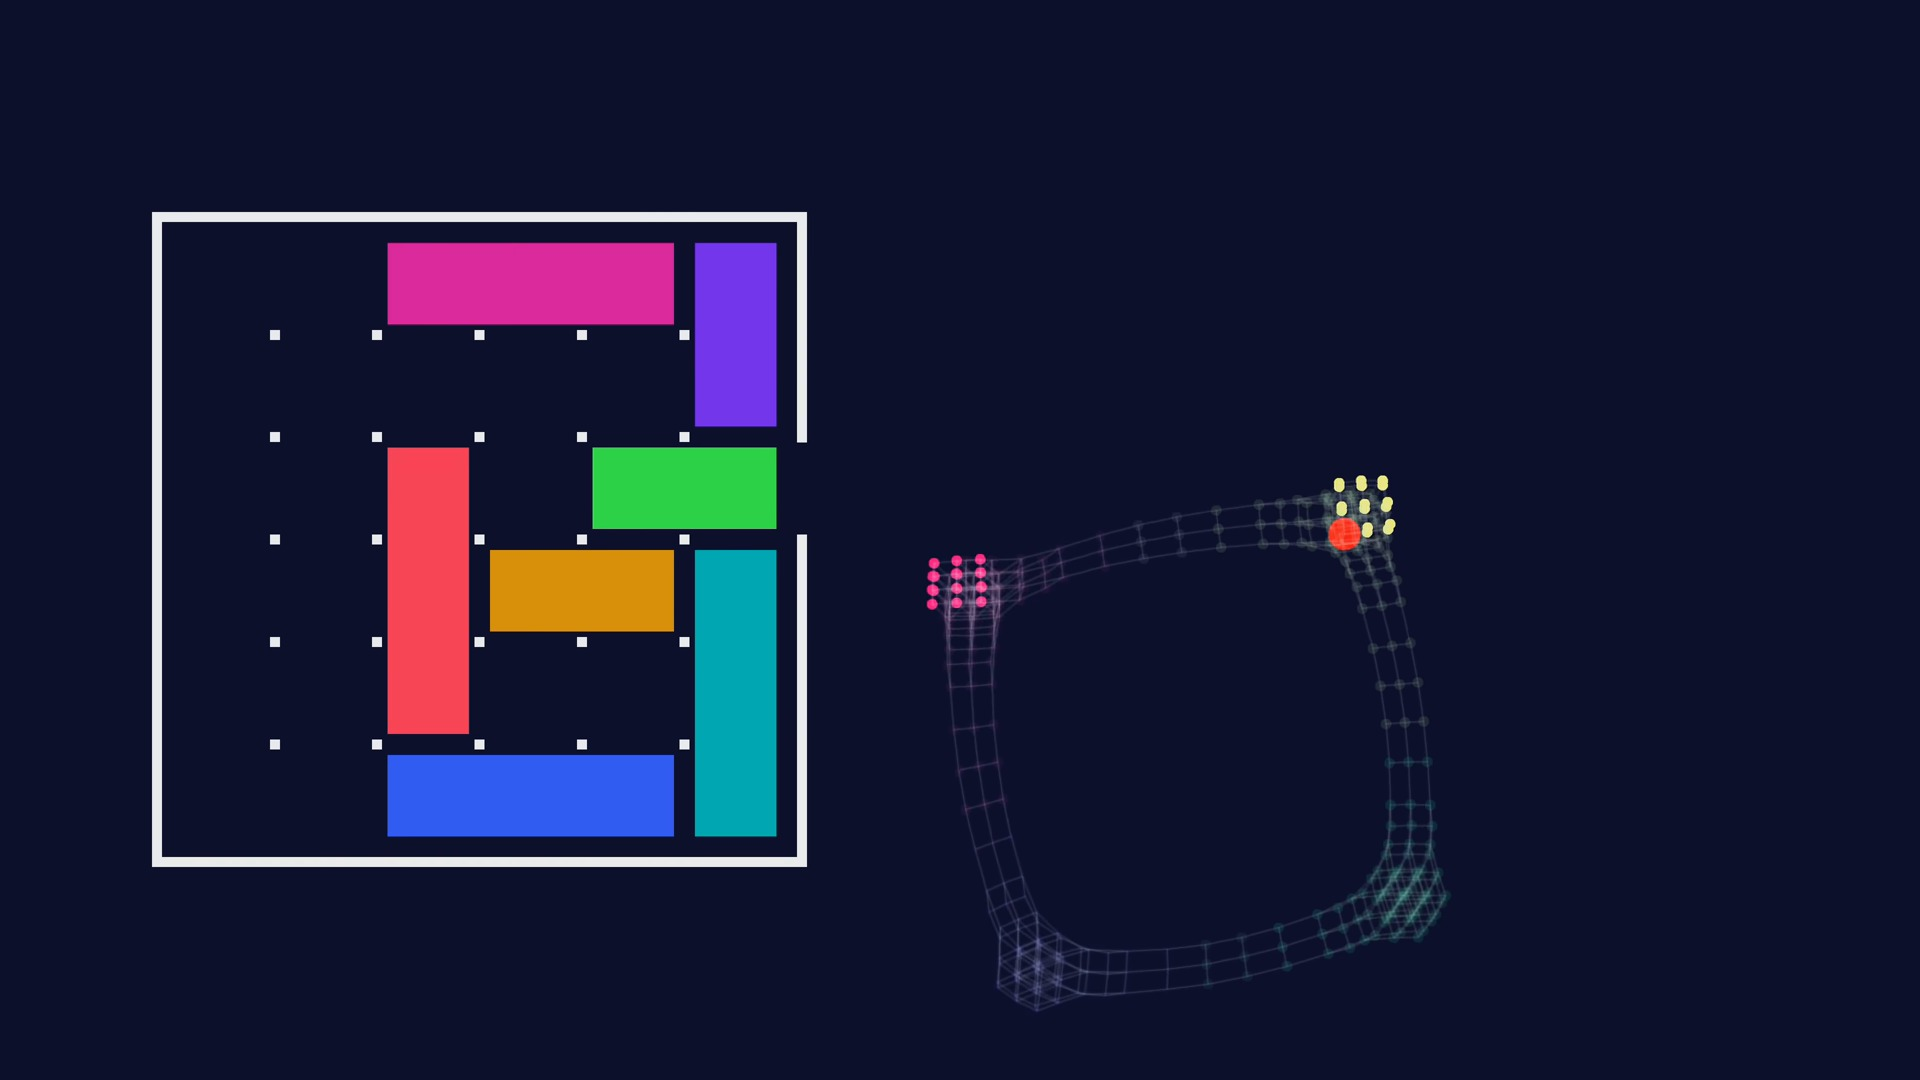
\includegraphics[width=0.90\textwidth]{figures/fig_15_solutions_corners.jpg}
\caption{黄点标出绿块已经靠在出口处的解；它们聚集在正方形中“绿块位于红杠右侧”的那些角落，当前节点以红点标出\vtag}
\end{figure}
\srcnote{00:04:59--00:05:14}
\end{minipage}

\subsection{本章小结}

竖直红杠把绿、橙两块锁进左右两种卡位，并且一次只放行一块，于是超结构成为四角正方形。解全部住在绿块已经越过红杠、贴着出口的那些角上。

\section{华容道的 25955 个节点：起点、解、密坑与细线}

现在回到华容道。目标是把那块最大的方块从底部开口移出去。它和上一道谜题有一处关键差别：交叉处没有销钉，块可以横向移动，因此难得多。上一道红杠谜题里，竖直红杠像销钉一样限制了过渡方向；华容道里没有这种销钉，块可以沿横向错开，状态空间因此不再是那座四角正方形，而会膨胀成一张大得多的图。讲者下班后把这盘题拿给同事，对方一直解到晚上 11 点才离开；同事觉得最难的一步，是把大方块挪到水平横杠下面。讲者自己倒不想先手解，他更想看这盘题“底盘里的形状”究竟是什么，以及“把盒子送到杠下”是不是真的最难。字幕在整图生成期间（约五分五十六秒到六分二十二秒）短暂没有解说，随后讲者报出节点总数。

\noindent\begin{minipage}{\textwidth}
\begin{figure}[H]
\centering
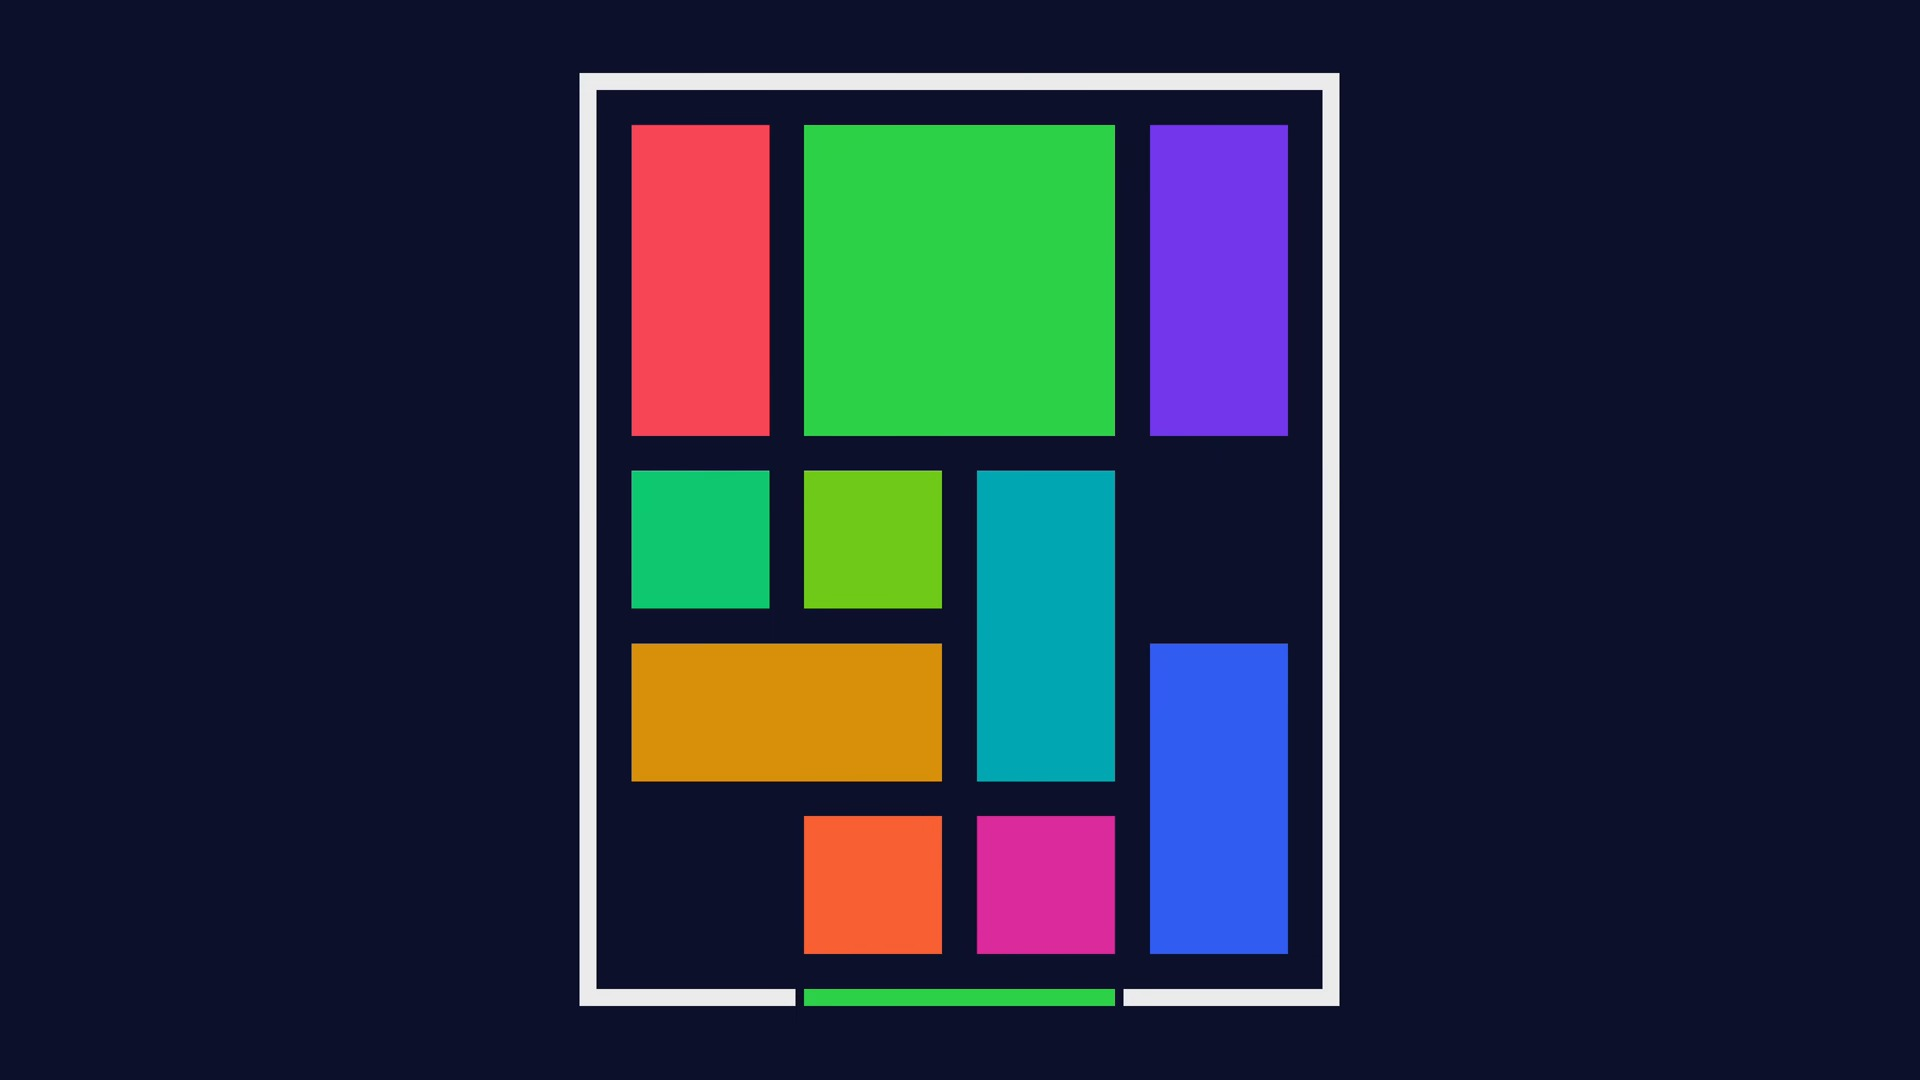
\includegraphics[width=0.90\textwidth]{figures/fig_16_klotski_goal.jpg}
\caption{华容道的目标：把顶部那块绿色大方块从底部开口移出；开口以底边的绿色标记示意\vtag}
\end{figure}
\srcnote{00:05:20--00:05:31}
\end{minipage}

把可达状态全部展开，得到 $25{,}955$ 个节点。谜题左右对称，图也左右对称：取某个盘面，总能在图的对面找到它的镜像。把图旋转九十度，还可以粗略看成两半。

\noindent\begin{minipage}{\textwidth}
\begin{figure}[H]
\centering
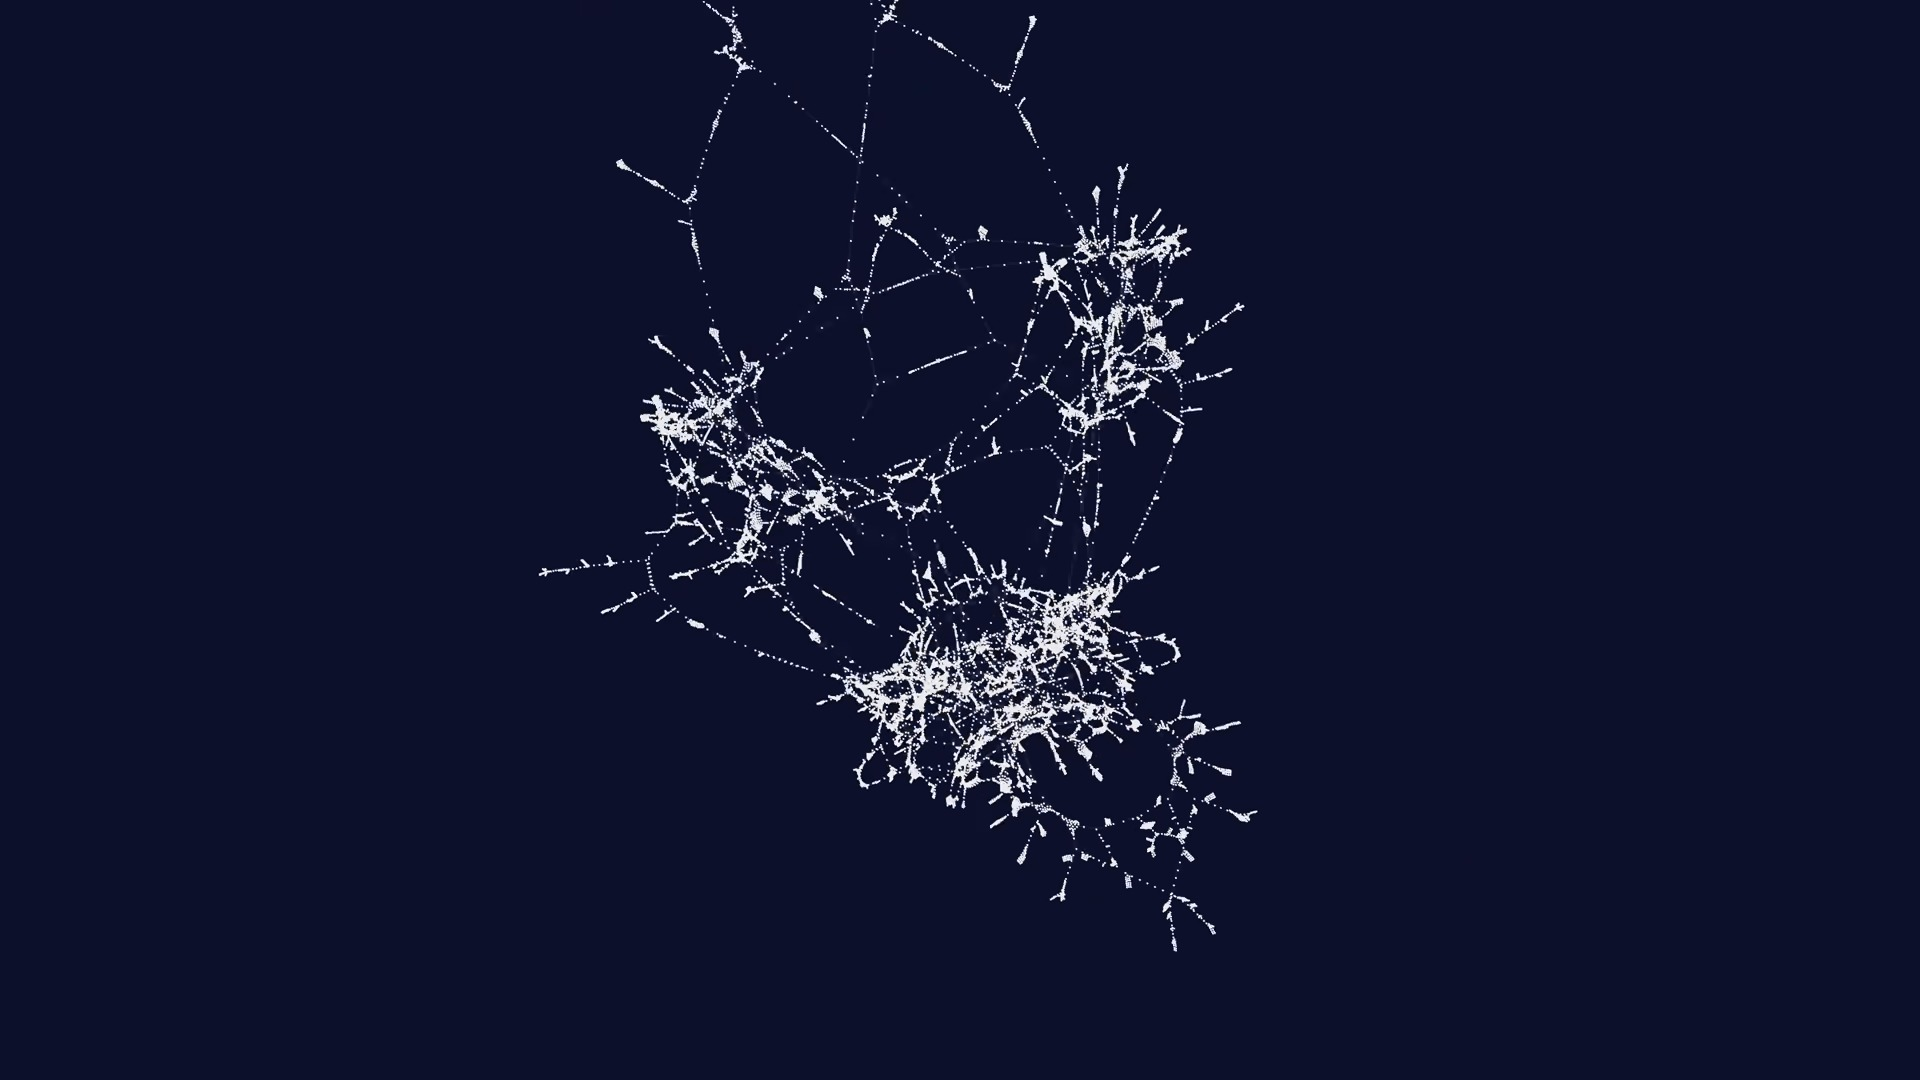
\includegraphics[width=0.90\textwidth]{figures/fig_17_nodes_25955.jpg}
\caption{华容道可达状态图的全貌，共有 $25{,}955$ 个节点\vtag}
\end{figure}
\srcnote{00:06:22--00:06:26}
\end{minipage}

\noindent\begin{minipage}{\textwidth}
\begin{figure}[H]
\centering
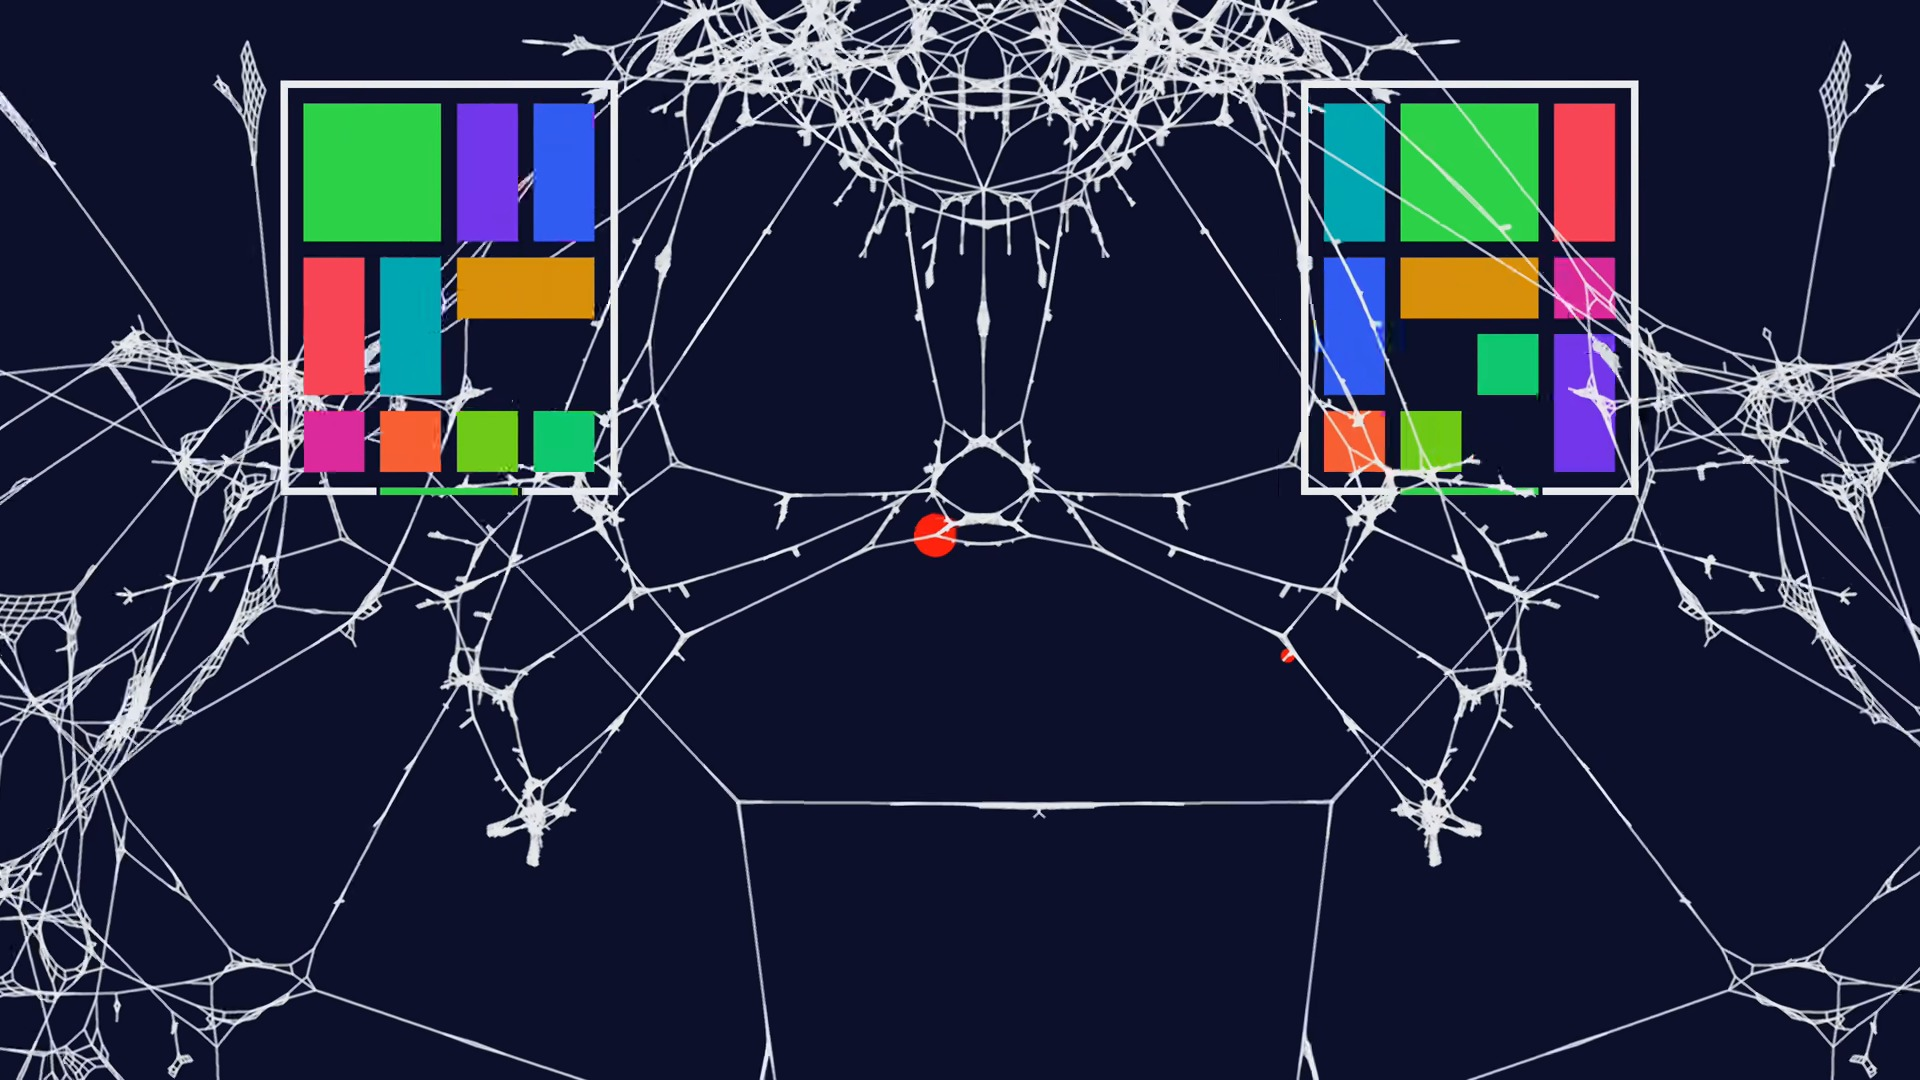
\includegraphics[width=0.90\textwidth]{figures/fig_18_mirror_symmetry.jpg}
\caption{左右两张盘面互为镜像，红点标出图上与之对应的位置；整张图随之左右对称\vtag}
\end{figure}
\srcnote{00:06:26--00:06:42}
\end{minipage}

红点是起始局面，青色标出的是大方块已经到达底部开口的全部解。所有解都住在与起点相反的那一半里。换言之，解题不是在起点附近打转，而必须走到图的另一侧。

\noindent\begin{minipage}{\textwidth}
\begin{figure}[H]
\centering
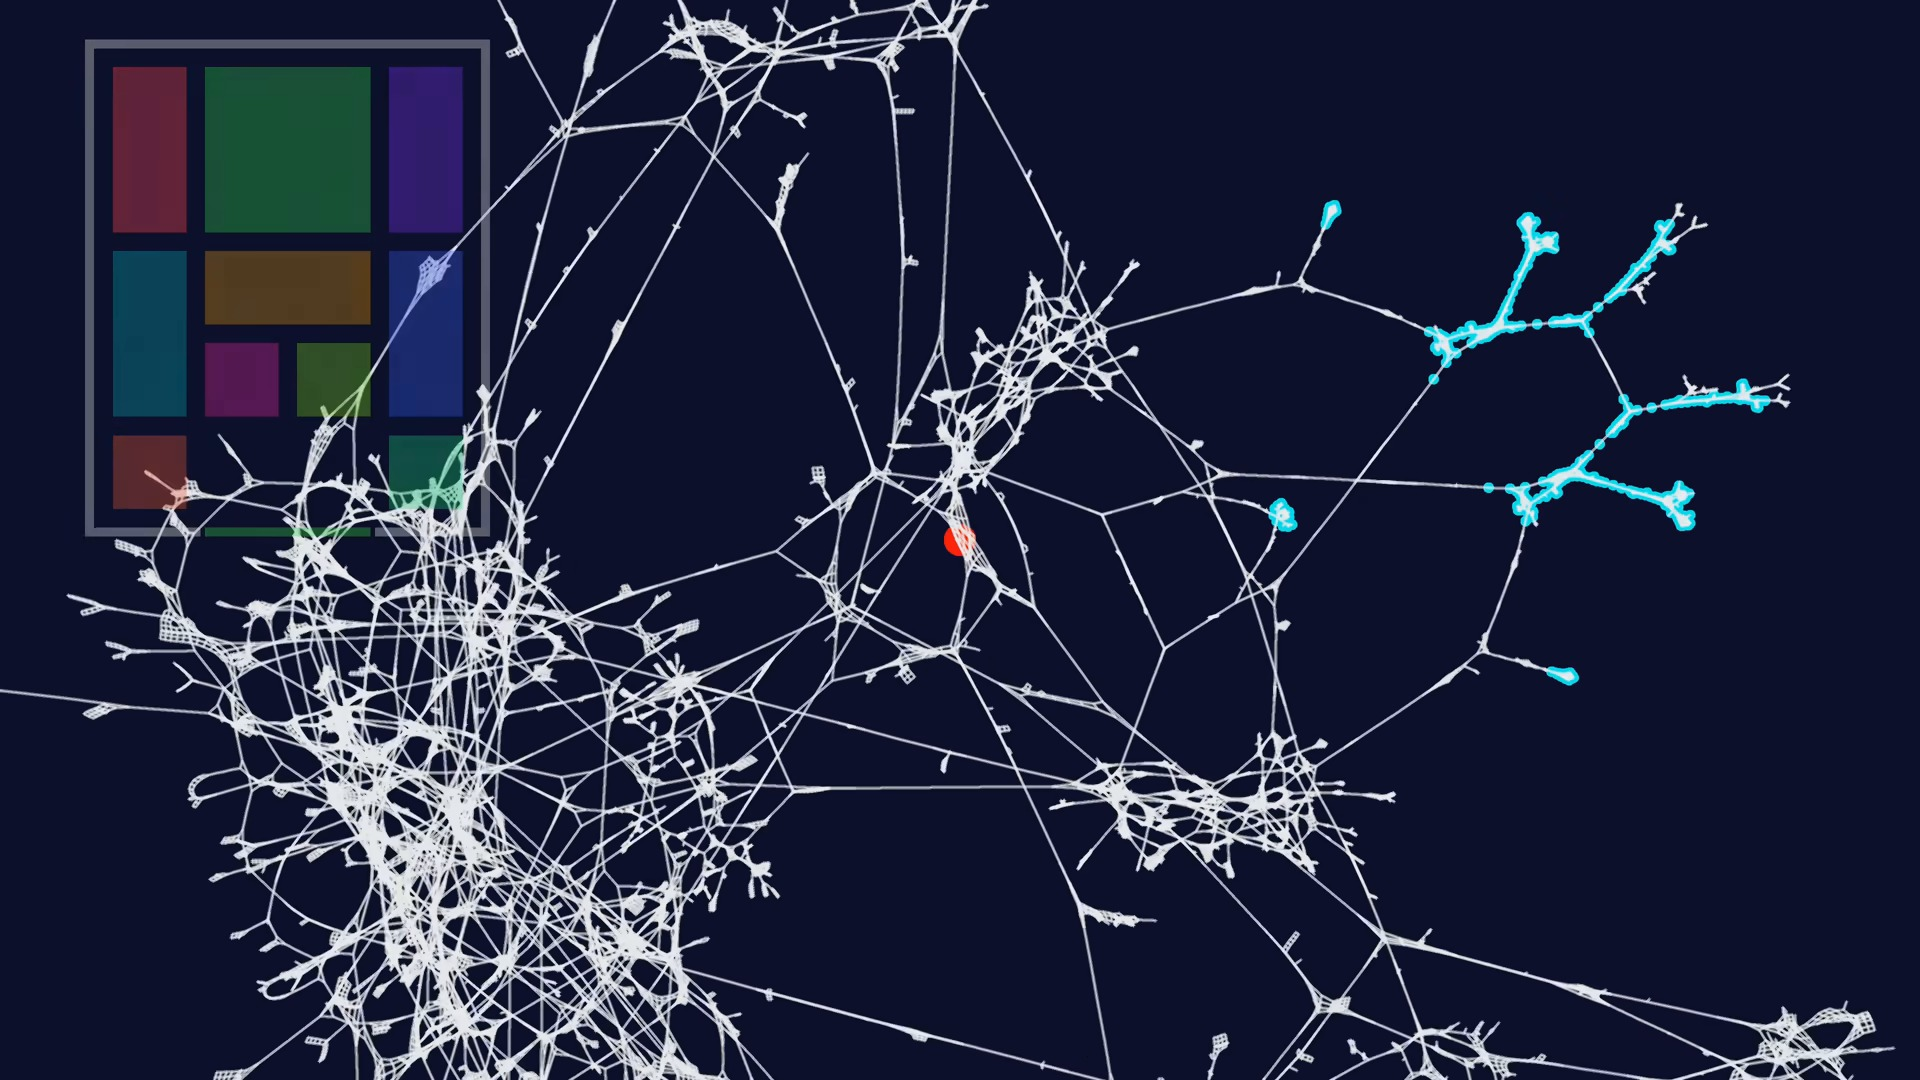
\includegraphics[width=0.90\textwidth]{figures/fig_19_start_vs_solutions.jpg}
\caption{红点为起点，右侧青色分支为解集（大方块已在底部）；两者分居状态图的两半，左上角淡出起始盘面\vtag}
\end{figure}
\srcnote{00:06:47--00:06:55}
\end{minipage}

若只做随机滑动，除非运气很好，多半会掉进一片特别稠密的“坑”里。要从起点到对侧，真正可行的办法是沿着某几条非常细的走廊走。讲者标出其中一条，并说明这就是通往某个解的最短路。

\noindent\begin{minipage}{\textwidth}
\begin{figure}[H]
\centering
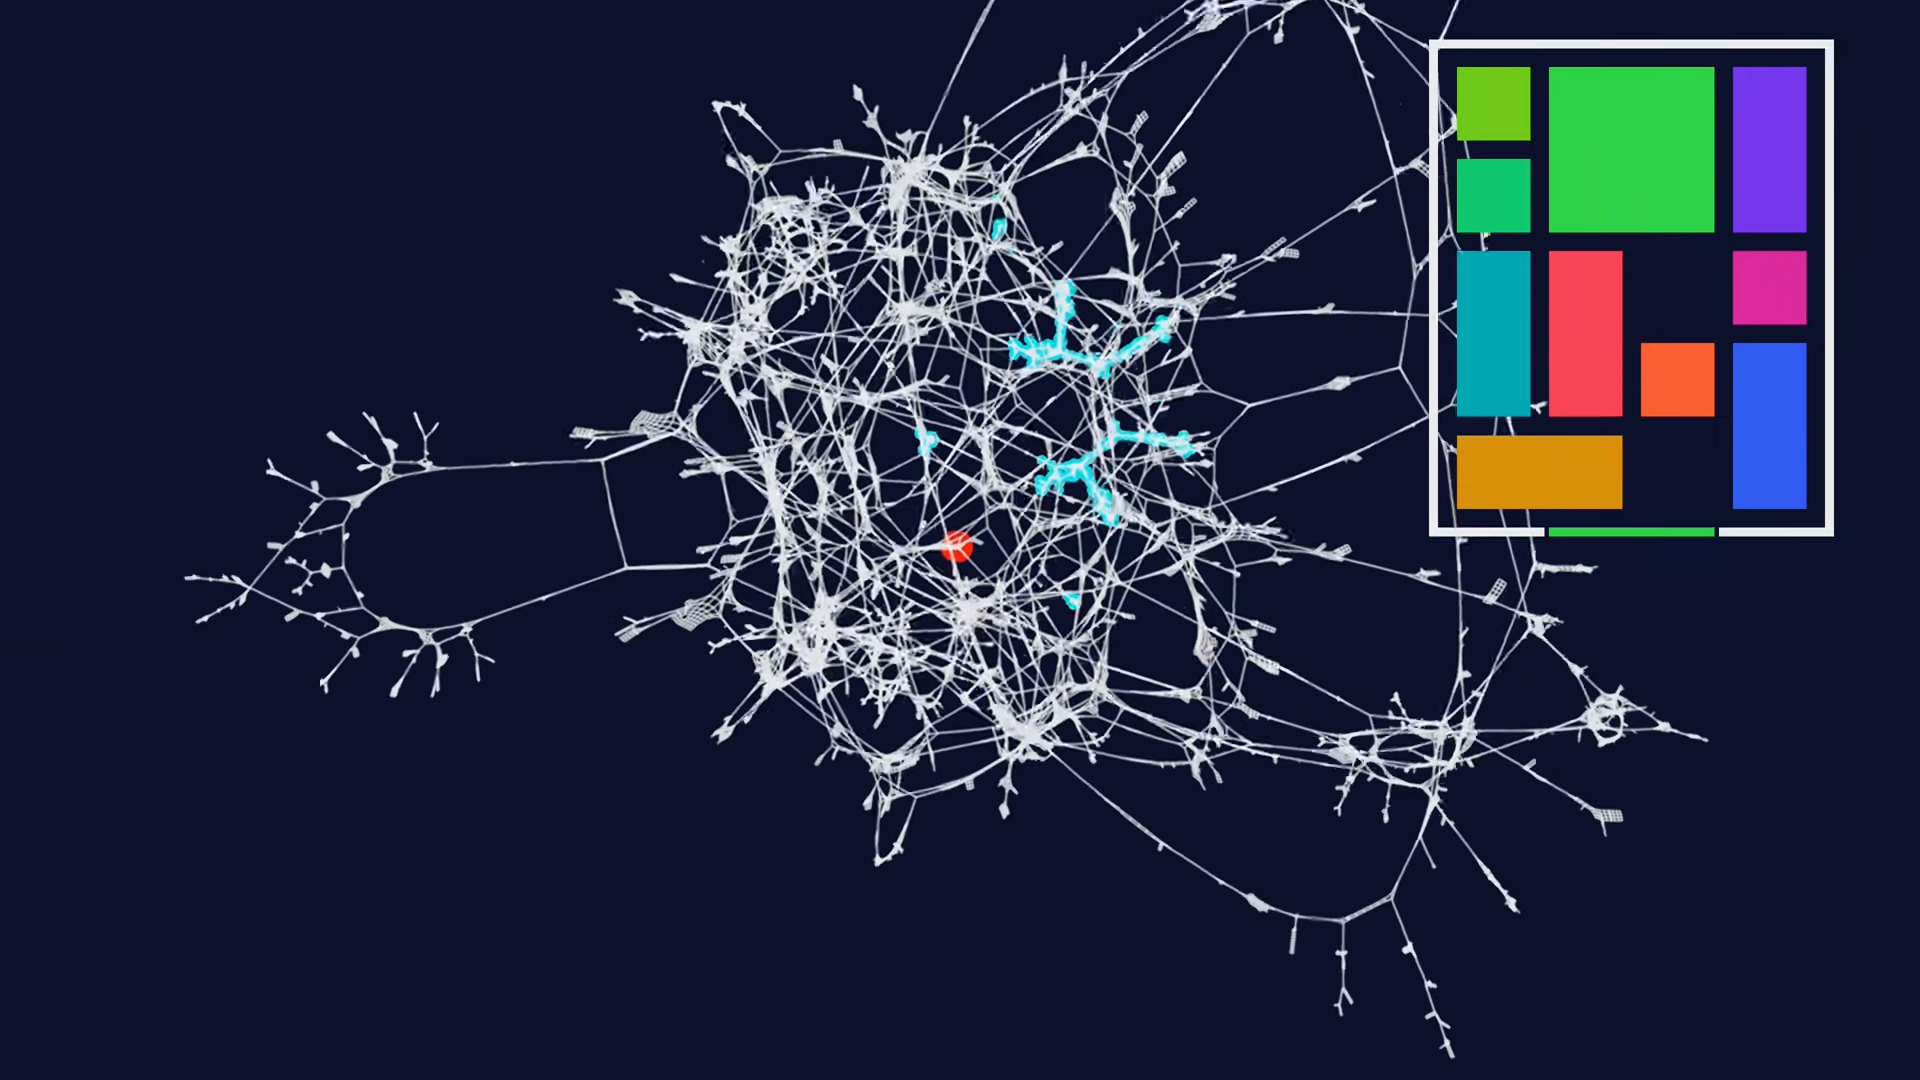
\includegraphics[width=0.90\textwidth]{figures/fig_20_dense_pit.jpg}
\caption{图中央出现一片高度缠结的稠密区域；随机游走很容易陷入这口“密坑”，红点为当前节点，青色仍是解集\vtag}
\end{figure}
\srcnote{00:07:01--00:07:12}
\end{minipage}

\noindent\begin{minipage}{\textwidth}
\begin{figure}[H]
\centering
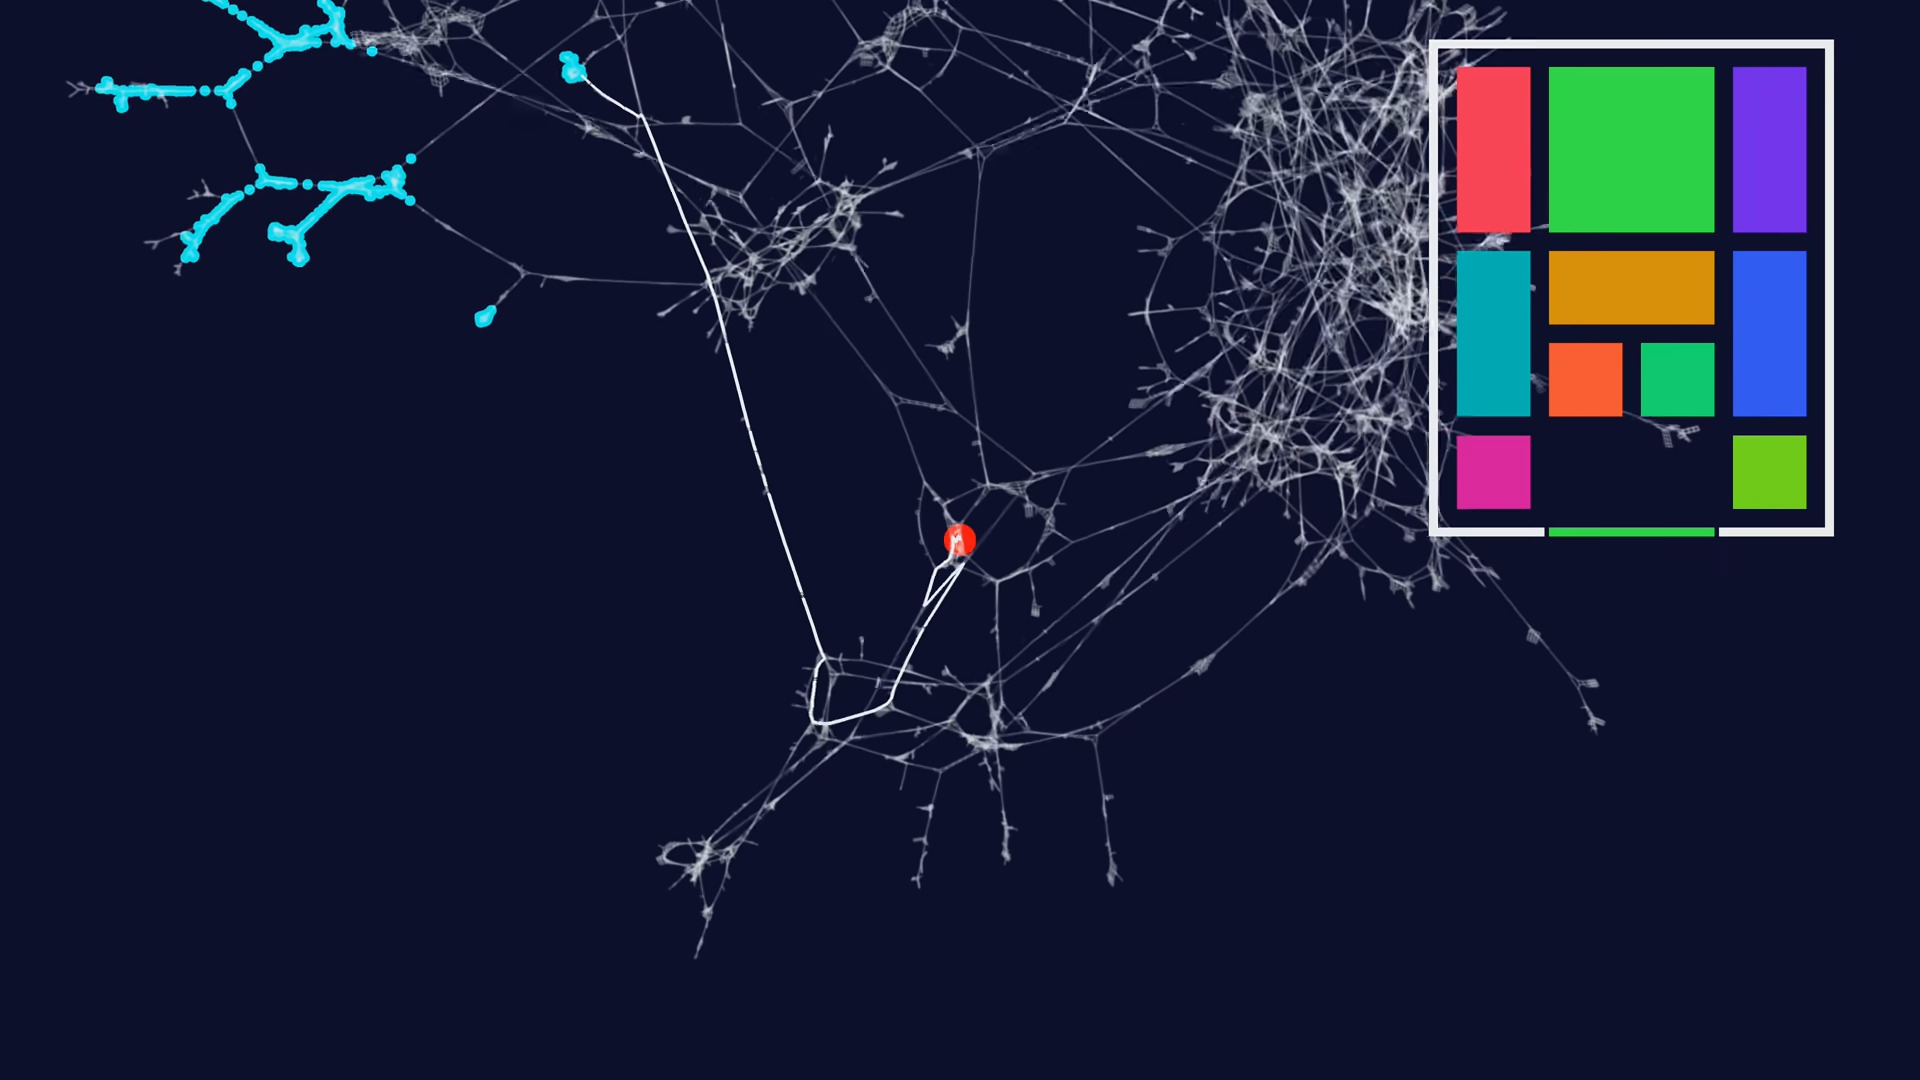
\includegraphics[width=0.90\textwidth]{figures/fig_21_shortest_path.jpg}
\caption{一条细白线从红点起点绕开密坑，通向左上方的青色解集：这是讲者标出的最短路\vtag}
\end{figure}
\srcnote{00:07:14--00:07:40}
\end{minipage}

有趣的是，吉尼斯世界纪录的速解选手并没有走这条最短路，而是走了另一条同样细、但路线不同的走廊。两条细线都能通到解，说明难处并不等于“只有一条路可走”，而是几乎所有宽阔的区域都不是通道，通道本身细得像线。随机智能体之所以显得在原地打转，正是因为它更常掉进密坑，而不是踩上这些细线。

\noindent\begin{minipage}{\textwidth}
\begin{figure}[H]
\centering
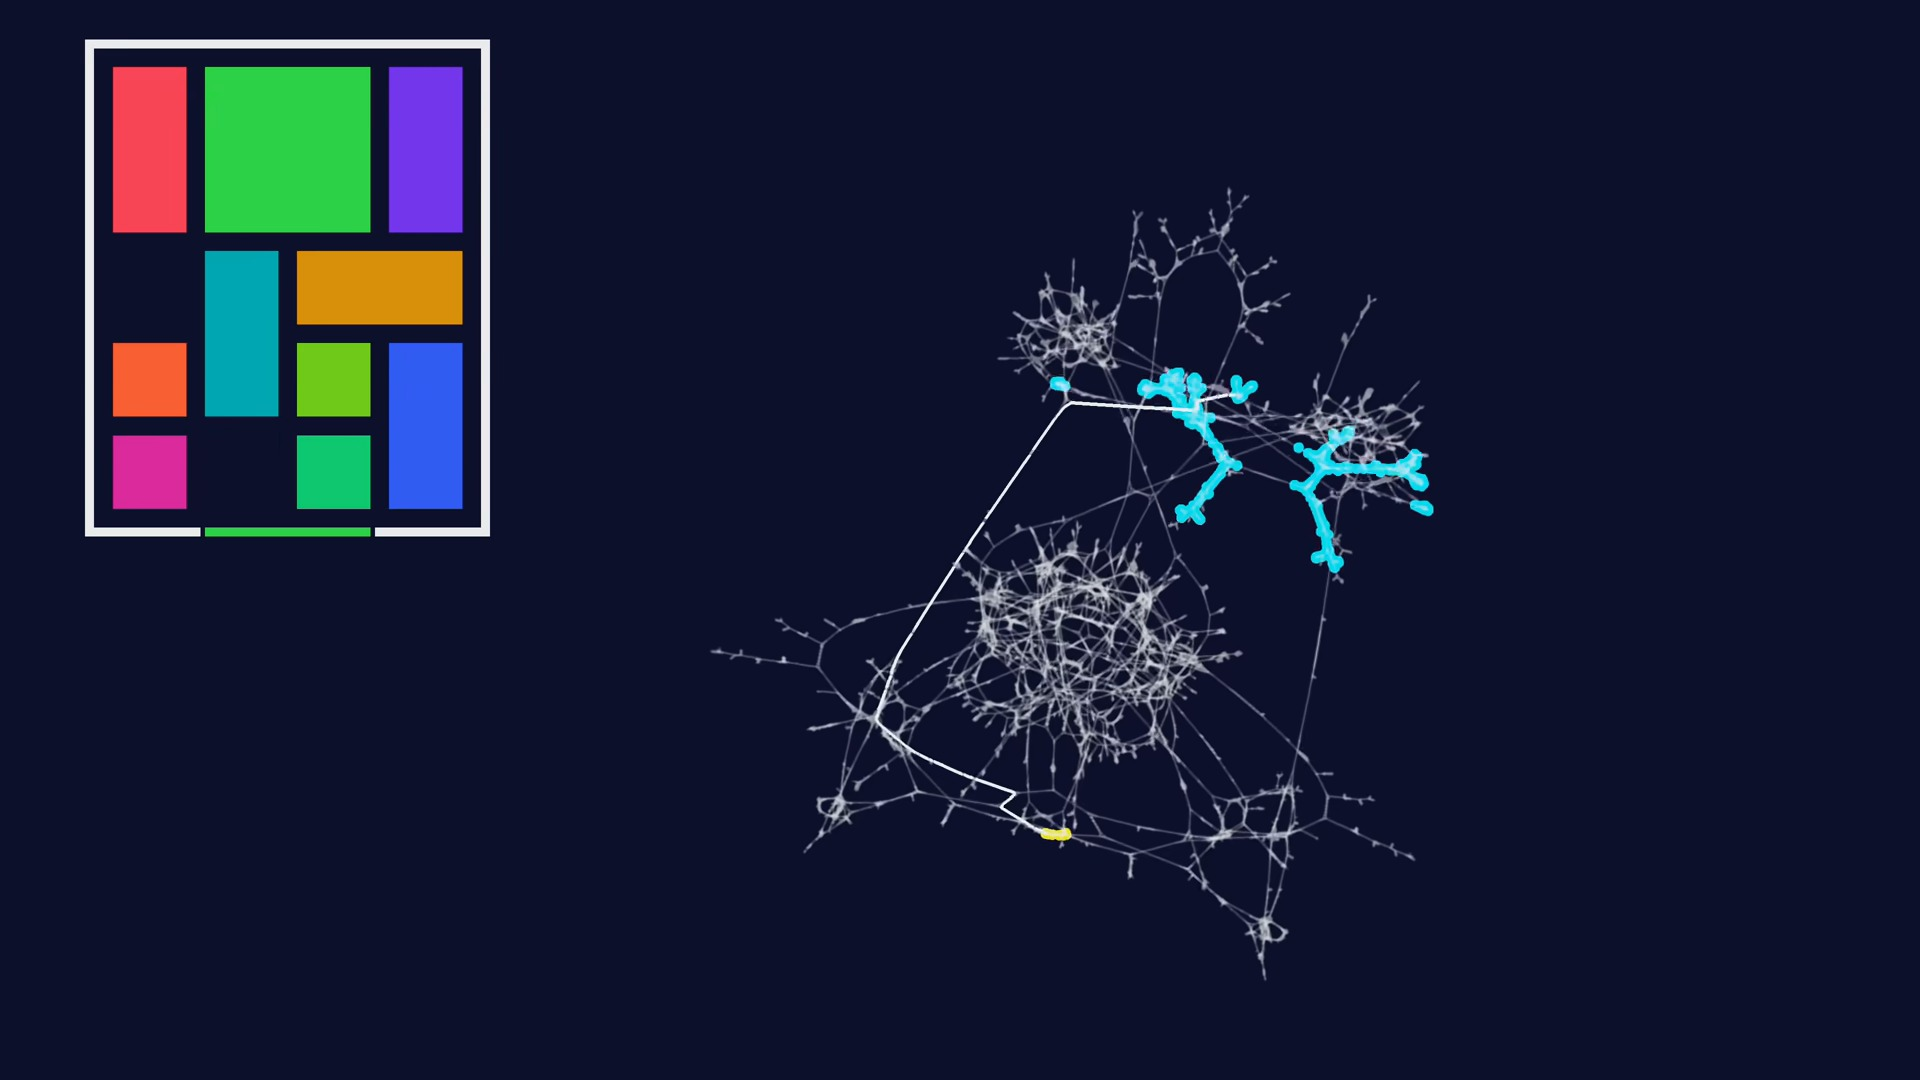
\includegraphics[width=0.90\textwidth]{figures/fig_22_gwr_path.jpg}
\caption{另一条细白线标出吉尼斯速解路线：它同样避开稠密区通往青色解集，却并不是最短路\vtag}
\end{figure}
\srcnote{00:07:40--00:07:53}
\end{minipage}

\subsection{本章小结}

华容道的可达图有 $25{,}955$ 个节点，左右对称，起点与解分在两半。随机走会掉进密坑，过关要沿细线走到对侧；最短路和速解纪录走的并不是同一条细线。

\section{把大方块移到横杠下面，是不是最难的一步？}

讲者用颜色给每个节点打标：红色表示大方块还在横杠上方，橙色表示二者已经并排，黄色表示大方块几乎要钻到杠下，绿色表示大方块终于到了横杠下方。再把解集叠上去，绿色区域与解集几乎重合。同事的直觉是对的：一旦方块到了杠下，离出口已经非常近；反过来，过不了这一步，就几乎到不了任何解。

\noindent\begin{minipage}{\textwidth}
\begin{figure}[H]
\centering
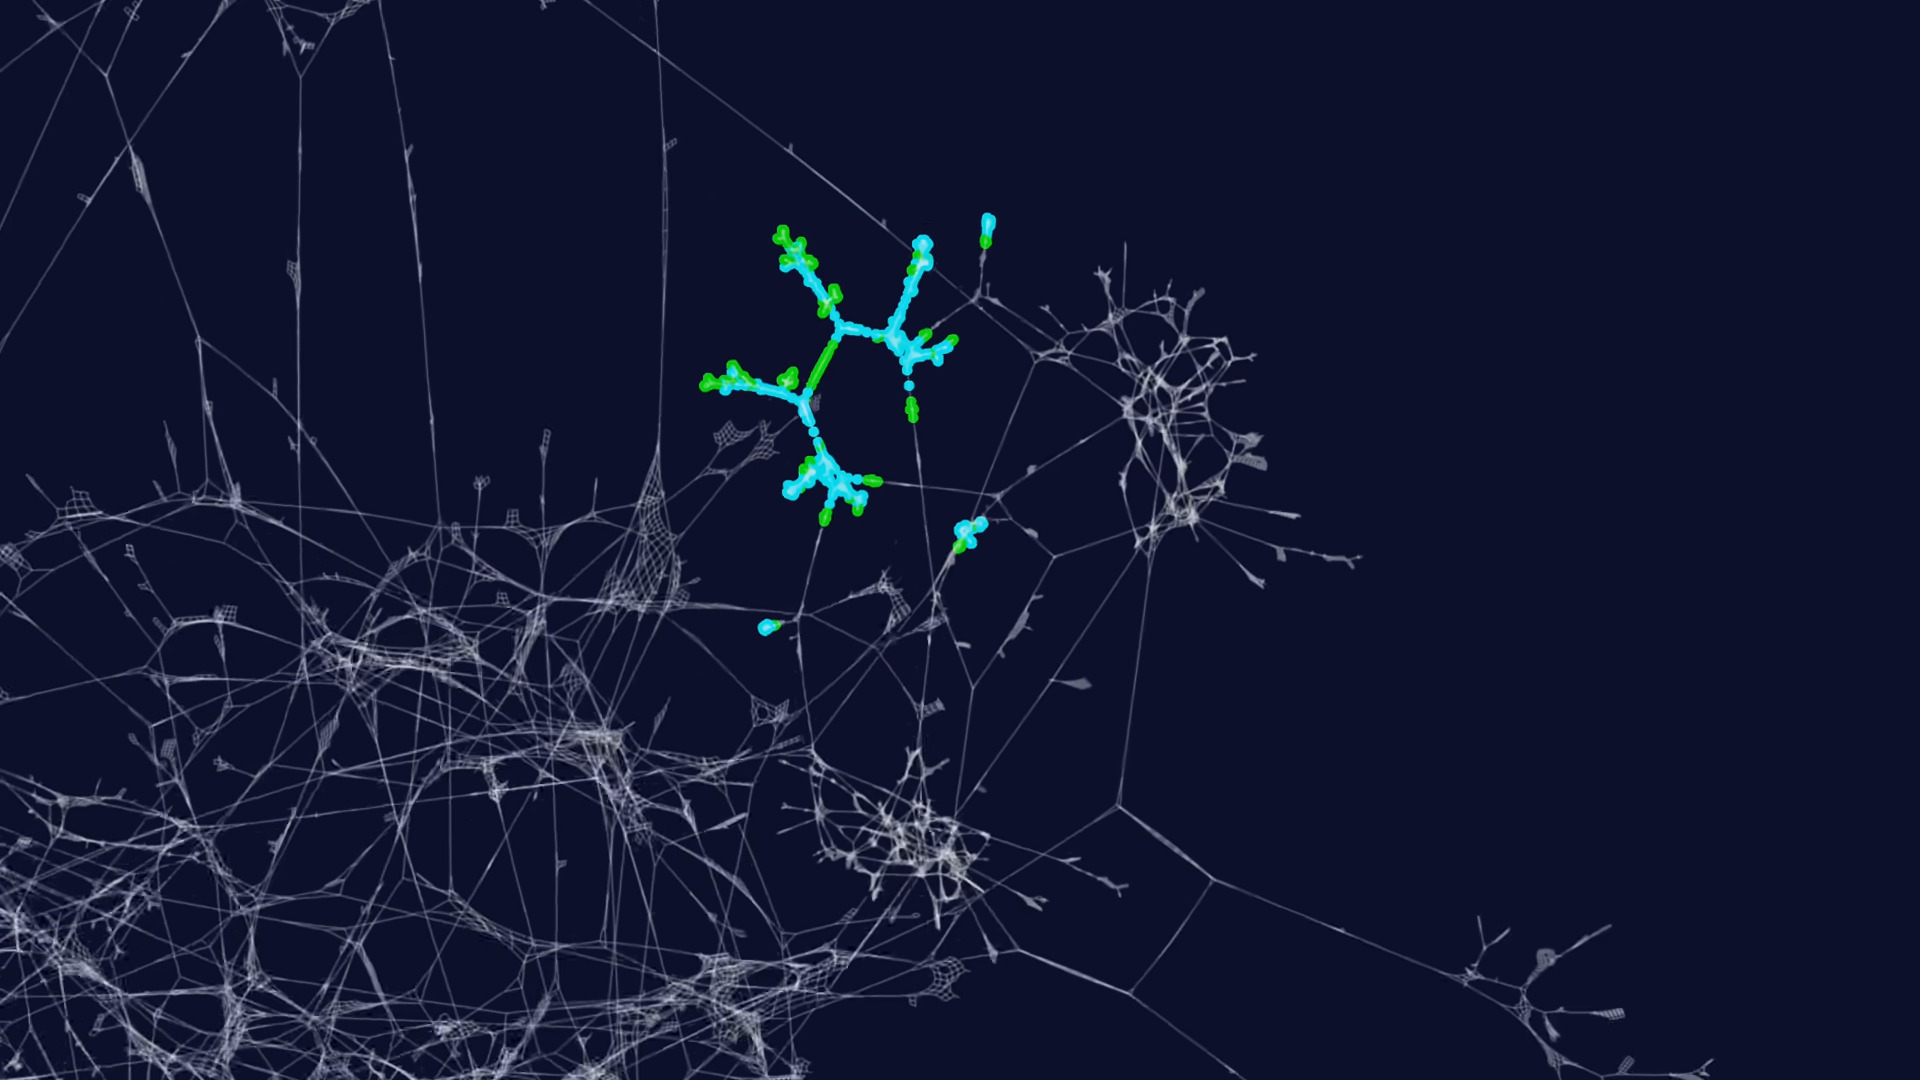
\includegraphics[width=0.90\textwidth]{figures/fig_23_overlap_solutions.jpg}
\caption{绿色节点表示大方块已在横杠下方，青色节点是解集，二者高度重叠\vtag}
\end{figure}
\srcnote{00:08:12--00:08:23}
\end{minipage}

\begin{importantbox}{这盘题真正难在何处}
若只看“随机滑动会不会成功”，难处是必须沿细线跨到图的另一半，并躲开密坑。若问“哪一种盘面变化几乎等于解题”，答案与同事的手感一致：把大方块送到水平横杠下方。这两句话描述的是同一张图上的不同切片，并不互相取消。
\end{importantbox}

\section{为什么只有左右对称？还有哪些互不相连的岛？}

图是左右对称的，却不是上下对称的。理论上，把所有块上下翻转，似乎也应得到一套合法盘面；实际上，除非把某一块拿出来再放回去，否则到不了那套翻转局面。把翻转盘面以及从那些盘面出发所能到达的全部节点补进图中，才得到兼具水平和竖直对称的“双重对称”图。原先那 $25{,}955$ 个节点，只是这座更大图里的一个连通分量。

\noindent\begin{minipage}{\textwidth}
\begin{figure}[H]
\centering
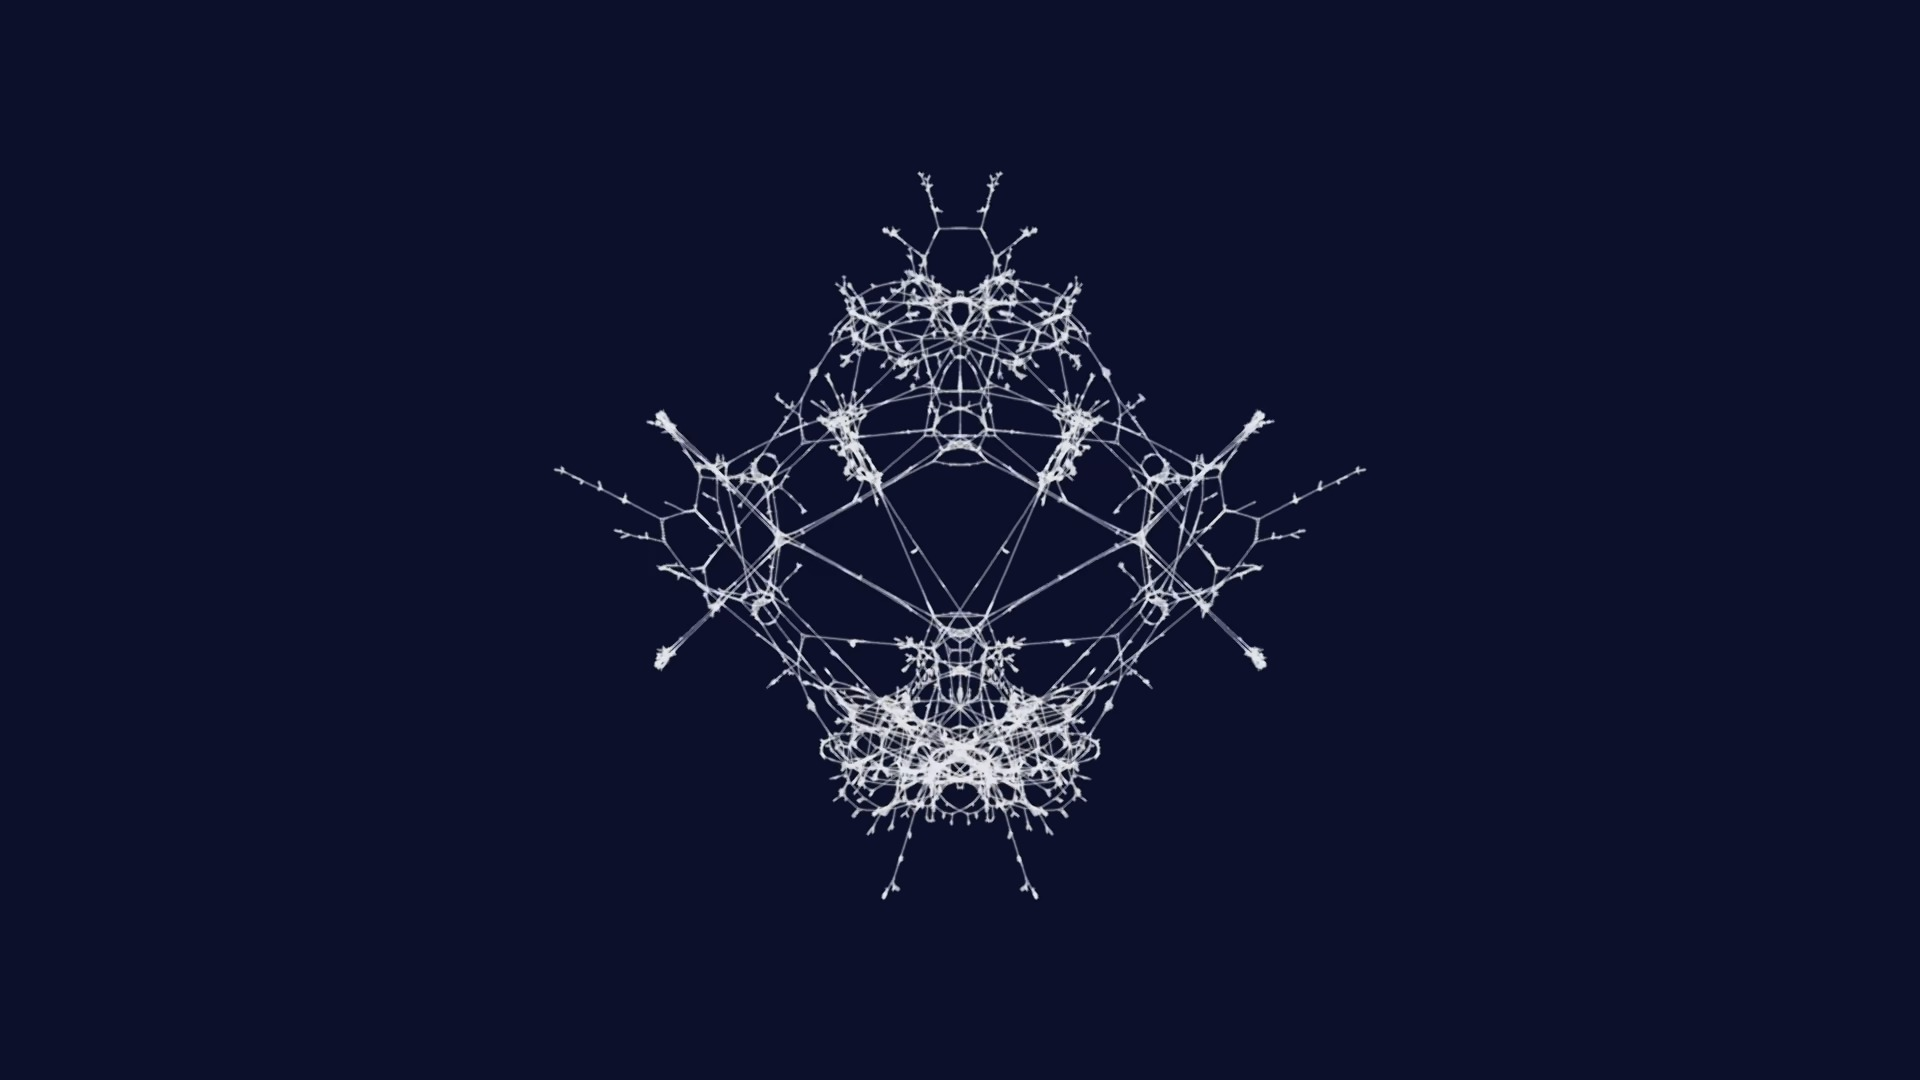
\includegraphics[width=0.90\textwidth]{figures/fig_24_doubly_symmetric.jpg}
\caption{补上翻转盘面及其可达部分之后，状态图呈现水平和竖直两个方向的对称\vtag}
\end{figure}
\srcnote{00:08:43--00:08:59}
\end{minipage}

除此之外，还有没有别的互不相连的岛？相当多。其中最大的一座只有 $248$ 个节点，主体是一条长路，偶尔分出短枝。和主分量那两万多个节点相比，这些岛既小又细，说明“拿起一块再放下”不只隔开了上下翻转，还隔开了许多更零碎的规则岛屿。

\noindent\begin{minipage}{\textwidth}
\begin{figure}[H]
\centering
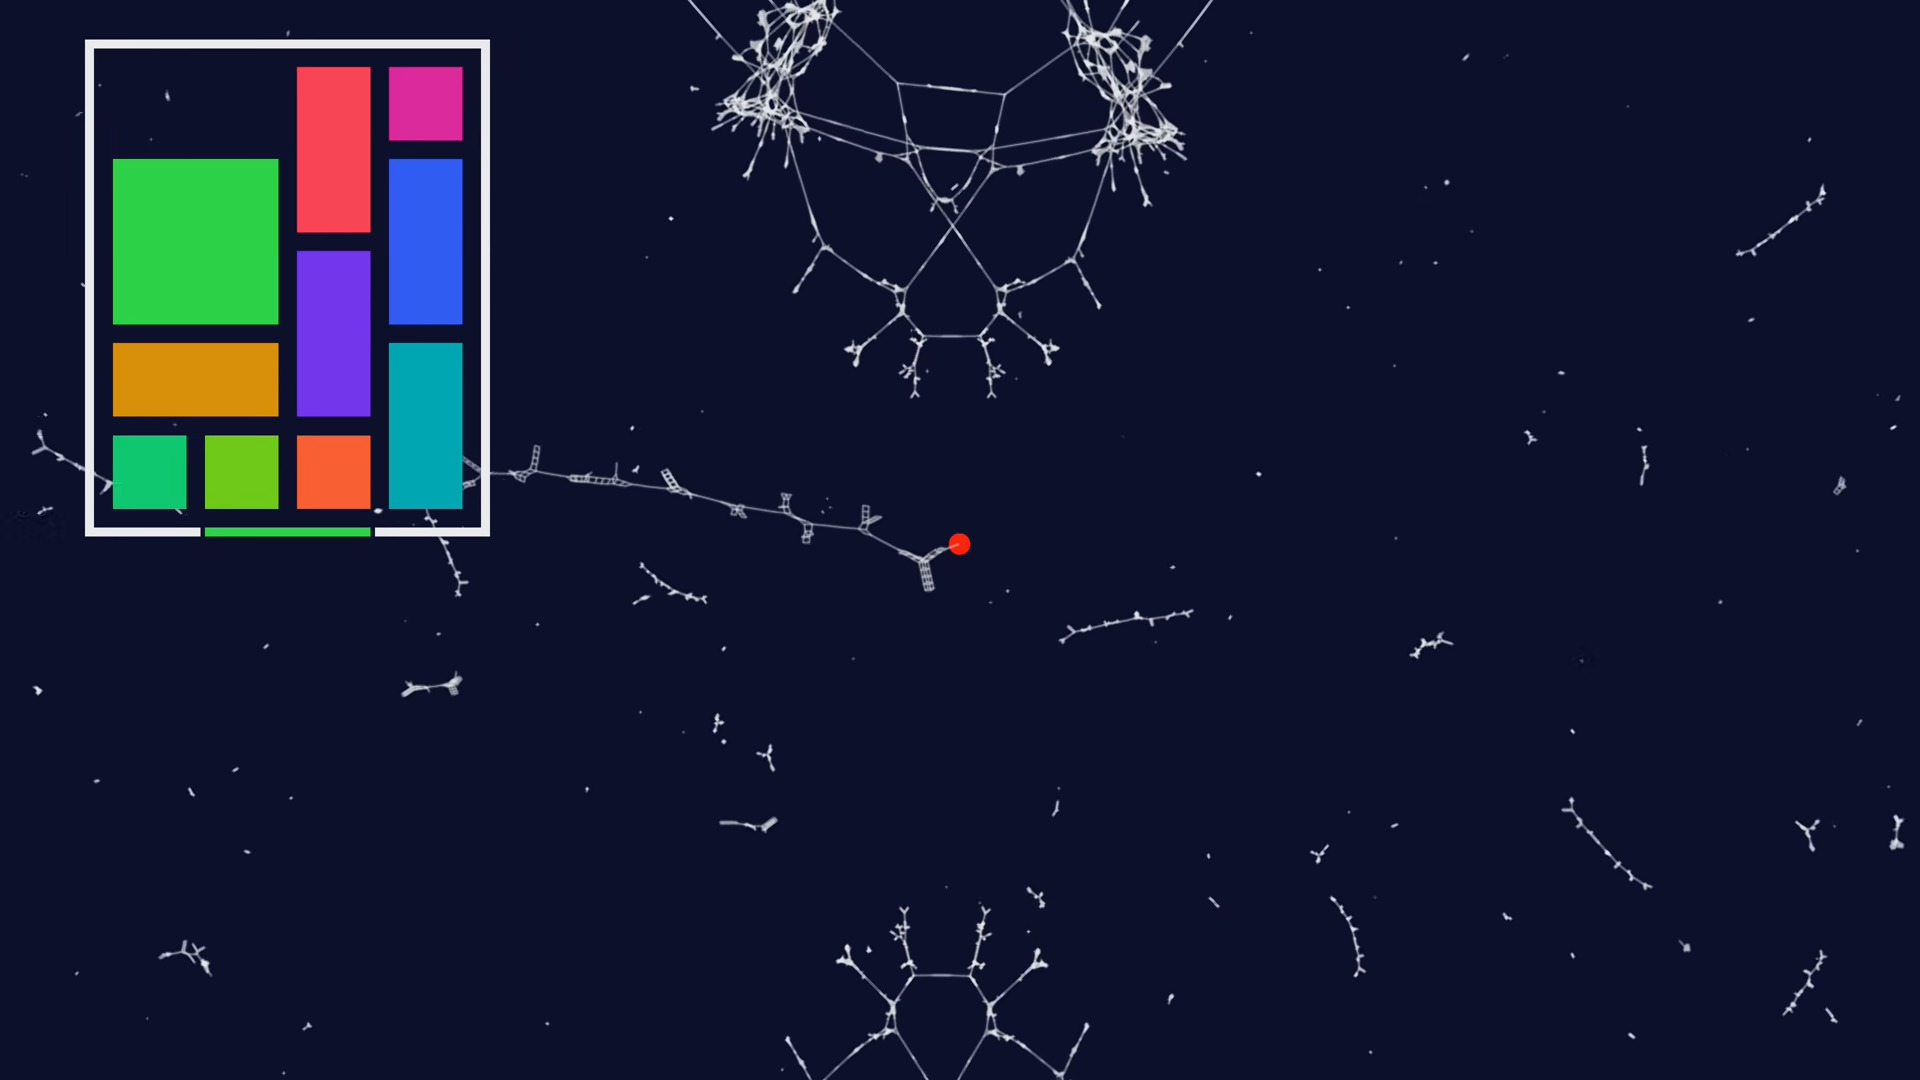
\includegraphics[width=0.90\textwidth]{figures/fig_25_island_248.jpg}
\caption{最大的不相连孤岛约有 $248$ 个节点，形态以一条长路为主，旁侧还有若干更小的碎片；左上角是该分量中的一个盘面\vtag}
\end{figure}
\srcnote{00:09:02--00:09:14}
\end{minipage}

\begin{warningbox}{不要把 25955 当成“全部合法摆法”}
$25{,}955$ 统计的是\emph{当前这块可达分量}里的节点。上下翻转、以及其他必须靠“拿出一块再放回”才能进入的局面，住在别的连通分量里。最大的一座岛只有 $248$ 个节点。
\end{warningbox}

\subsection{本章小结}

左右对称来自盘面本身的镜像；上下翻转则不可达，除非把一块拿出来。补上翻转分量后图才双重对称，此外还有许多小岛，最大者仅 $248$ 个节点。

\section{更根本的难度：许多局部子谜题被松散缝合}

讲者认为，只说“跨过两半很难”或“把方块送到杠下很难”，都还不够。他在图上远处圈出一小片节点，再把这些节点对应的盘面叠在一起、故意弄模糊，只留下它们共享的图案：在这片局部里，大方块和横杠都位于盘面中央。这块局部结构同样由两个空洞撑起，很像前面见过的二维格子。

\noindent\begin{minipage}{\textwidth}
\begin{figure}[H]
\centering
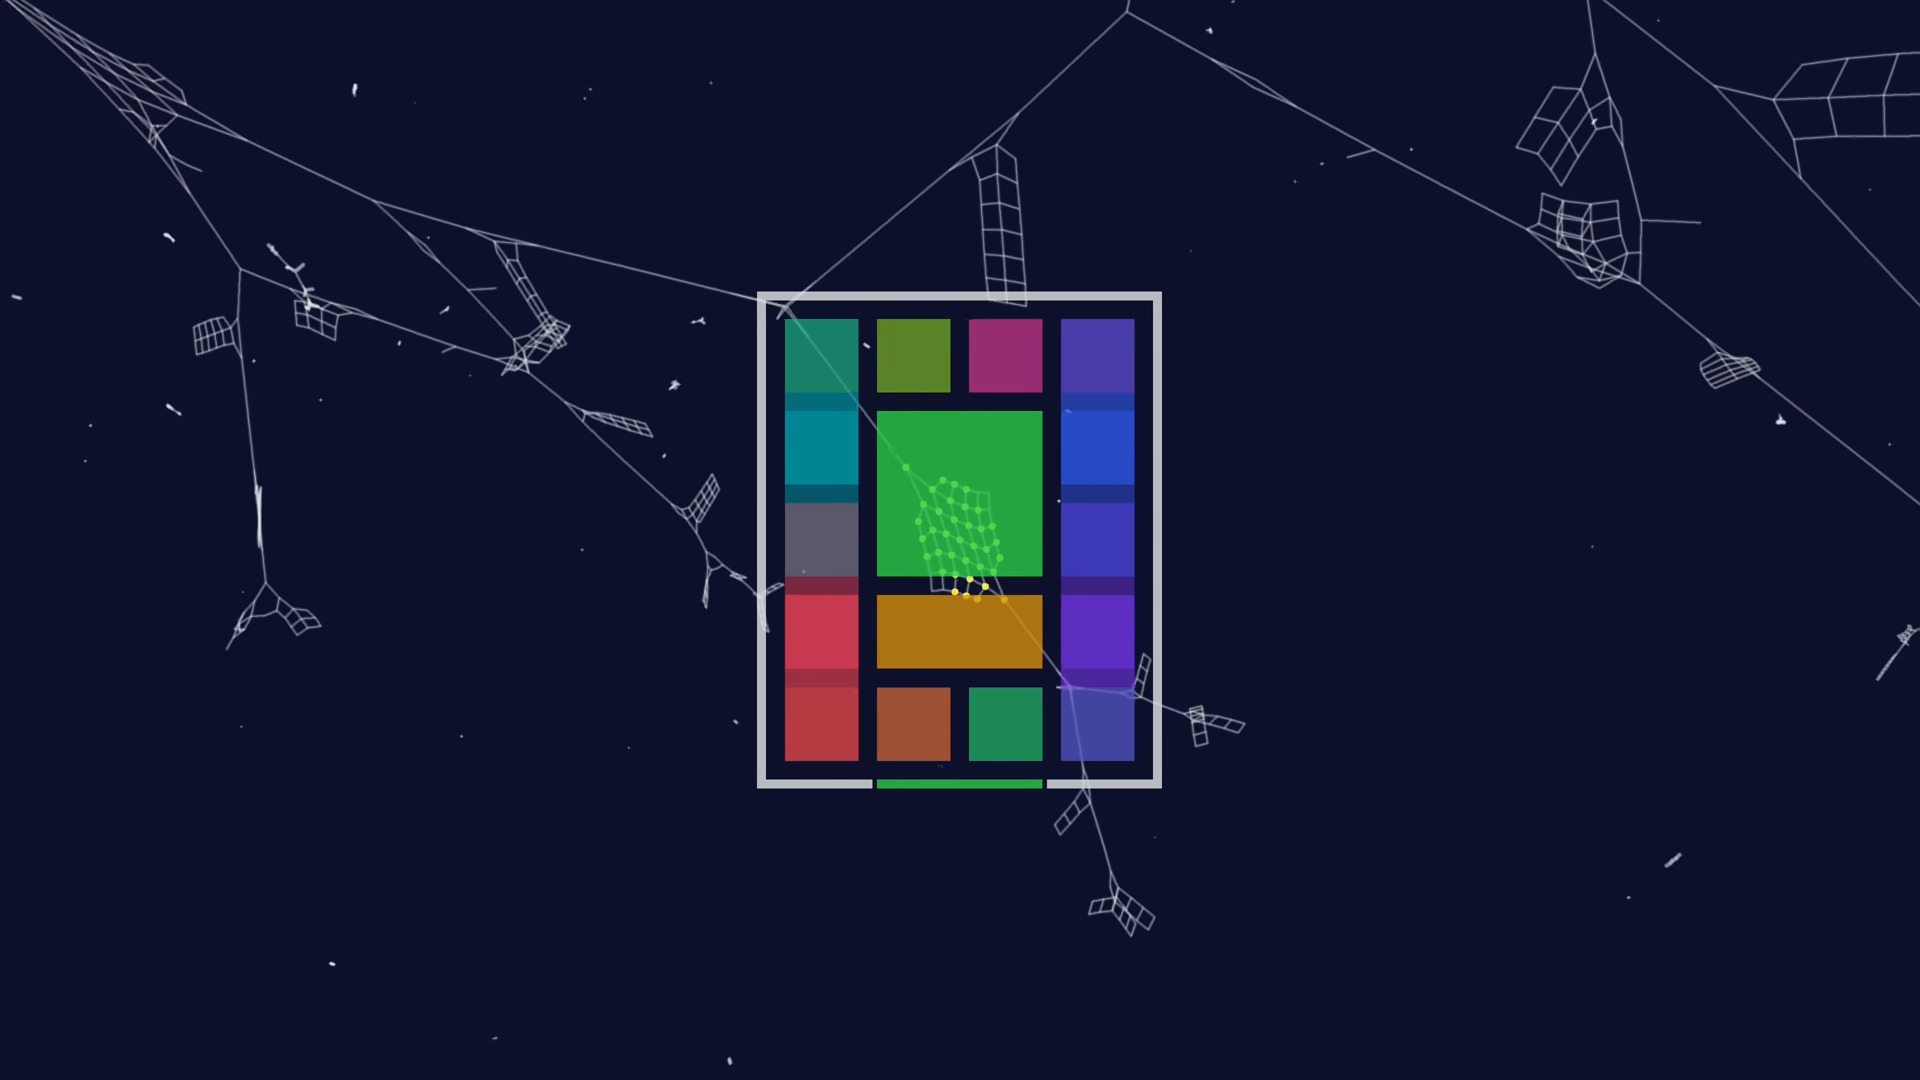
\includegraphics[width=0.90\textwidth]{figures/fig_26_blurred_shared.jpg}
\caption{把同一局部里许多盘面叠在一起并加以模糊后，共同特征显露出来：绿色大方块与橙色横杠都居中\vtag}
\end{figure}
\srcnote{00:09:40--00:09:53}
\end{minipage}

如果把两个空洞对齐到恰到好处的位置，就可以从当前这块局部“破出去”，进入另一套有自己规则与组织方式的子结构。

\noindent\begin{minipage}{\textwidth}
\begin{figure}[H]
\centering
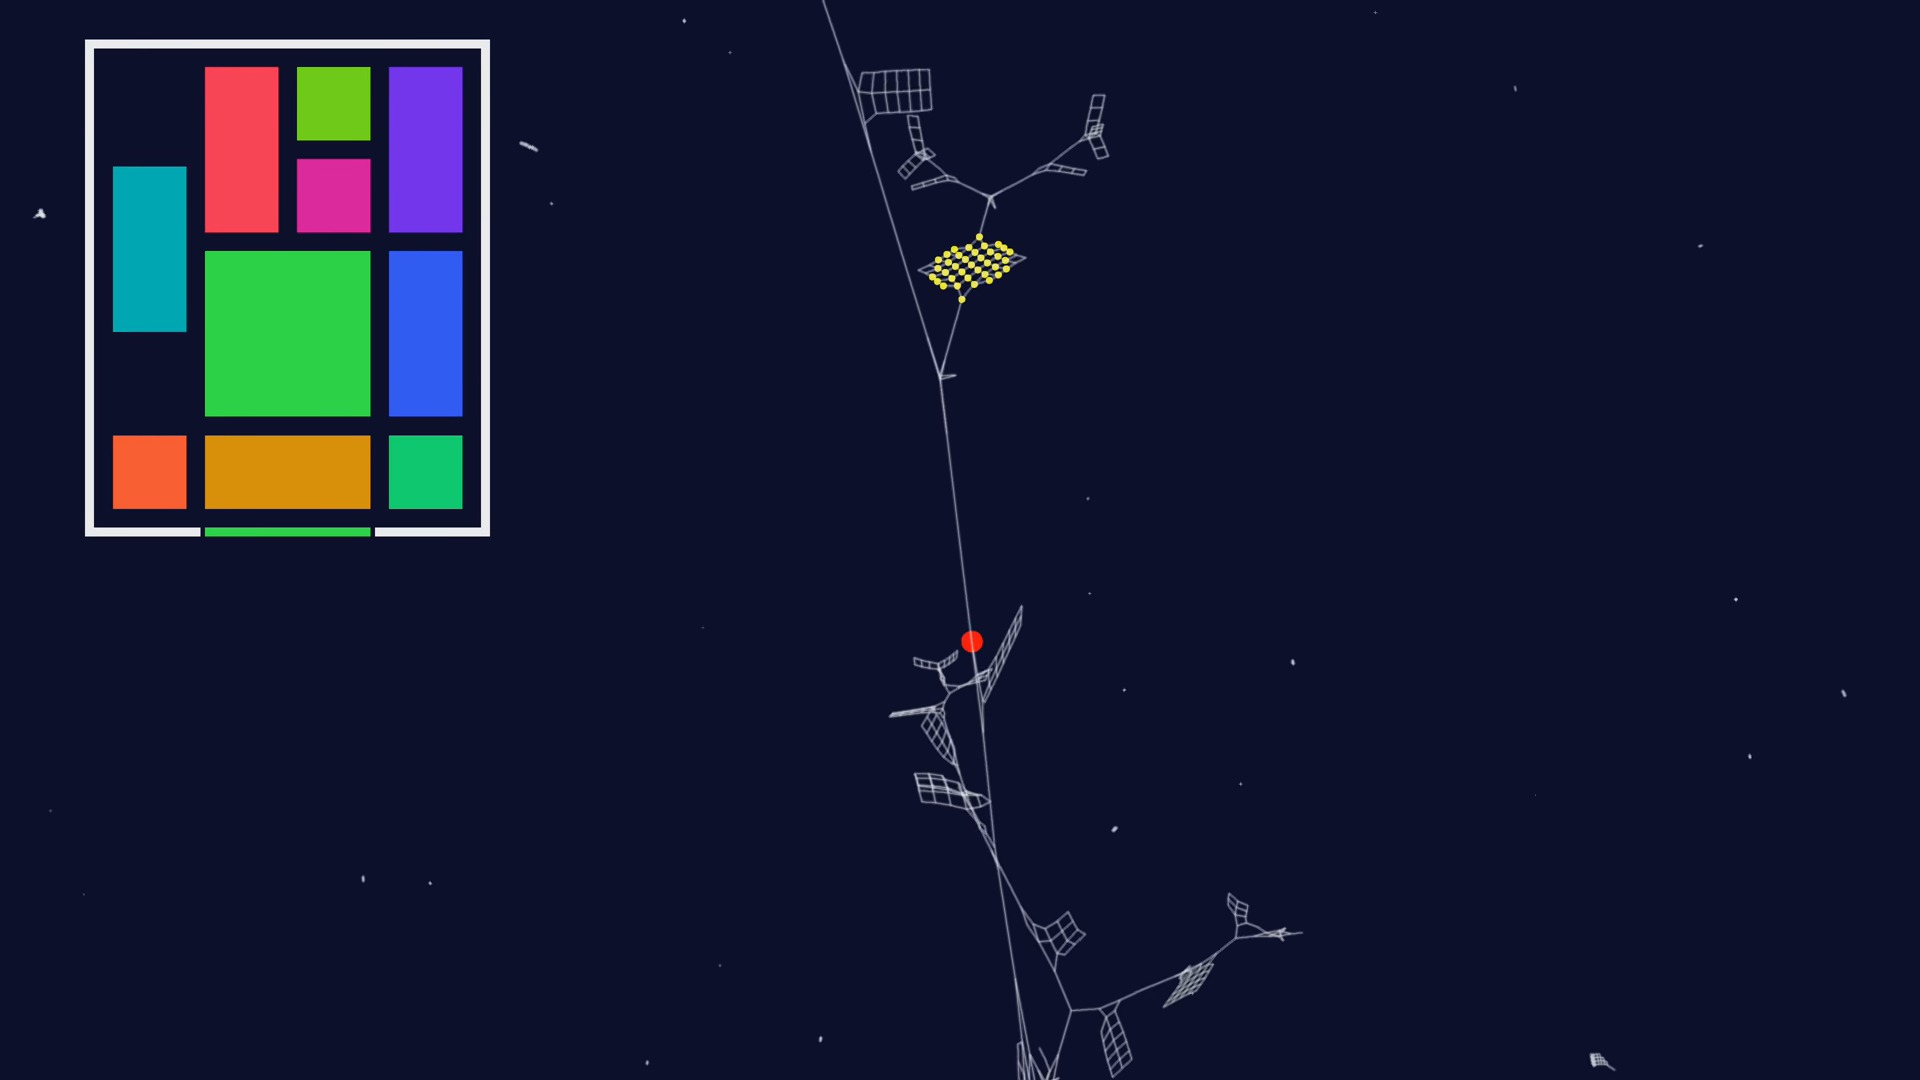
\includegraphics[width=0.90\textwidth]{figures/fig_27_breakout.jpg}
\caption{黄色高亮的小网格是由两个空位张成的局部二维结构；沿细线走到红点附近，就可以离开它，进入另一种组织方式\vtag}
\end{figure}
\srcnote{00:09:53--00:10:16}
\end{minipage}

\begin{importantbox}{不要把整张图当成单一拓扑}
讲者的概括是：华容道的状态图不宜理解成由一套统一规则统治的单一拓扑，而应看成许多局部子谜题的集合。每个子谜题有自己的逻辑和形态，它们被松散地缝合成一个大谜题。难度来自必须在这些局部规则之间找到缝隙、走过去。
\end{importantbox}

\section{总结：规则被穷尽之后，形态会自己长出来}

视频后段有一句几乎自嘲的话：这不过是个玩具，谁会在乎？讲者随即画出一个对照。观察自然世界时，我们会在最高处看到生物体的超结构，它通过多层抽象坐落在物理的子结构之上：生物体、细胞、分子、原子。分辨率上的这种分层，并不为物理学所独占；即便最日常的家用玩具也不例外。形态可以从对一套规则做计算式的穷尽探索里直接长出来。

\noindent\begin{minipage}{\textwidth}
\begin{figure}[H]
\centering
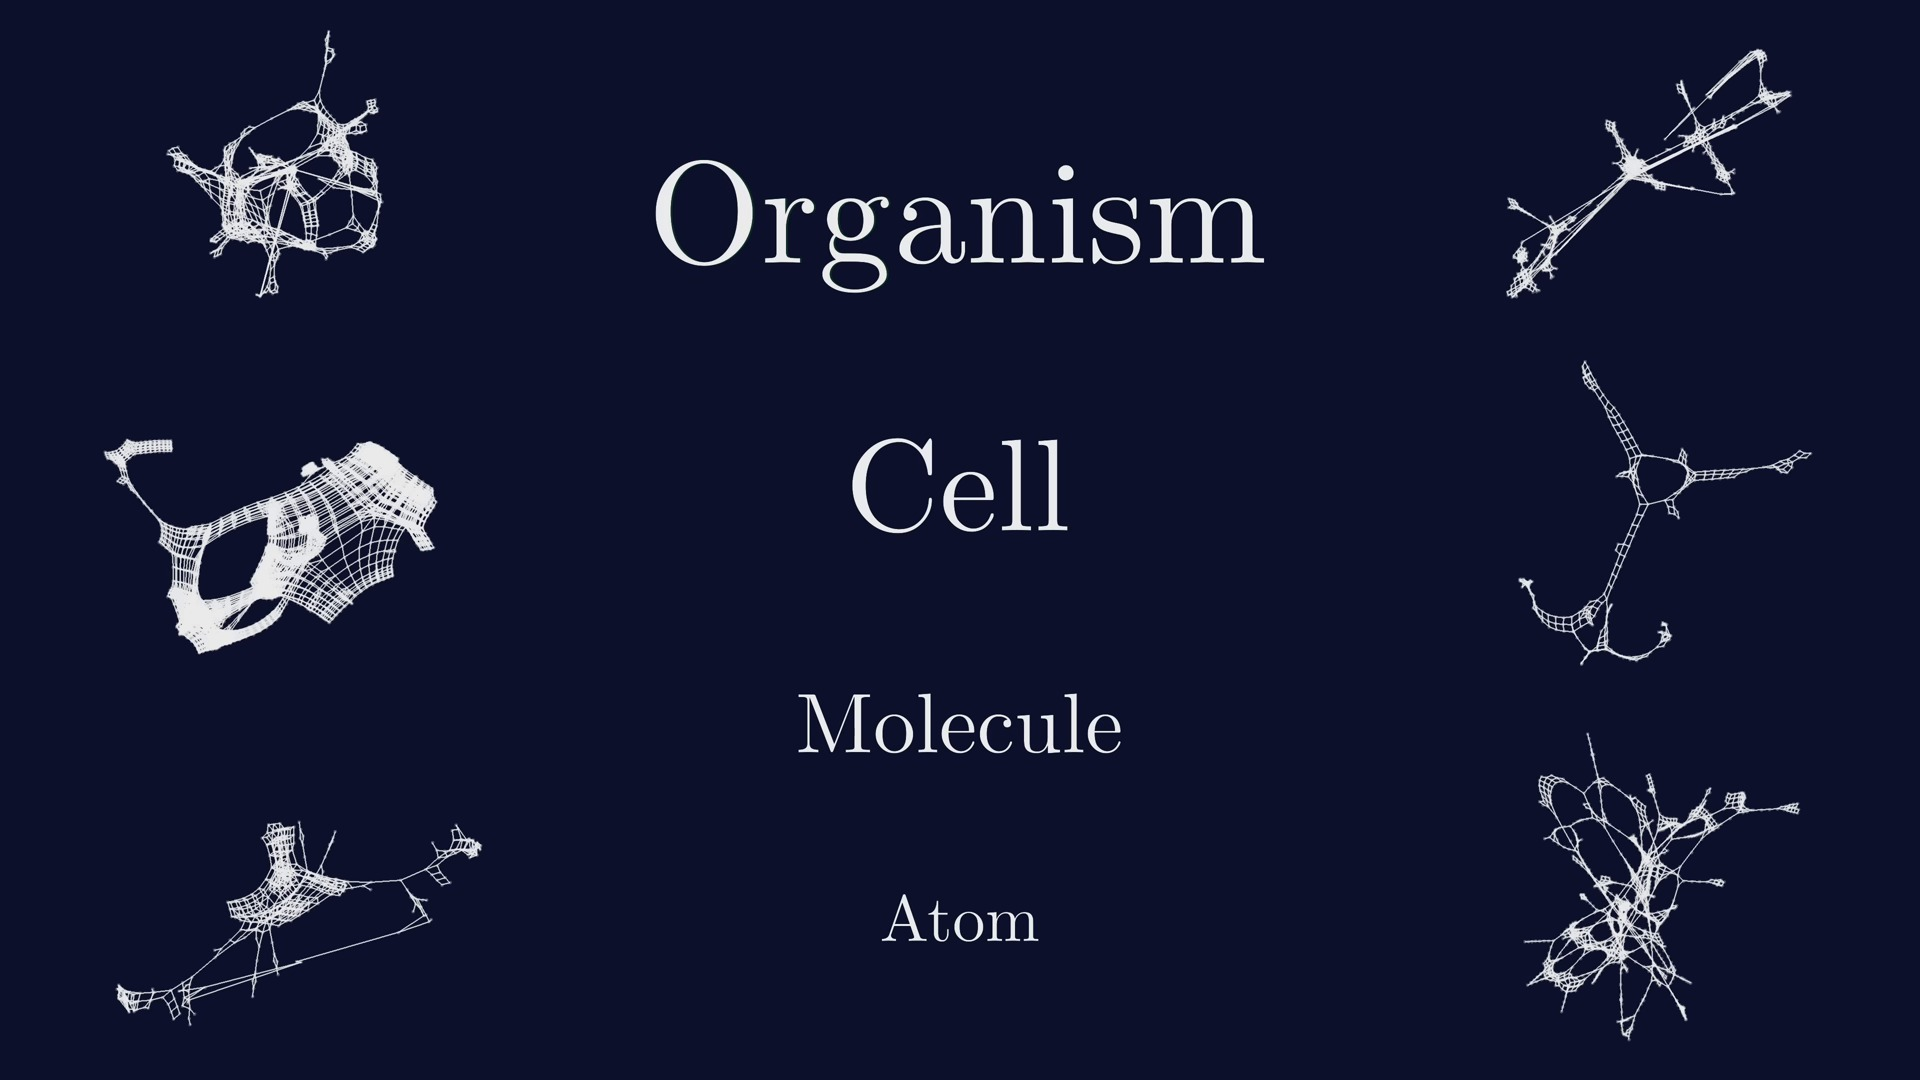
\includegraphics[width=0.90\textwidth]{figures/fig_28_bio_analogy.jpg}
\caption{讲者用 Organism、Cell、Molecule、Atom 四层名称，对照状态图在不同尺度上呈现的结构\vtag}
\end{figure}
\srcnote{00:10:44--00:11:10}
\end{minipage}

\begin{knowledgebox}{可以从这盘题带走的阅读方式}
以后再看滑动积木，不必只问“下一步往哪推”。更有收获的问题是：节点和边是什么；局部自由度由几块空位提供；哪些看起来合法的局面其实属于另一座岛；超结构把起点、解和“关键一步”分别放在图的哪一部分。华容道给出的具体数字是：$25{,}955$ 个可达节点，解与起点分居两半，大方块到横杠下方与解集几乎重合，另有一座仅 $248$ 个节点的长路孤岛。
\end{knowledgebox}

把前面的参照例子收成三条对照，便于记忆，但它们都是讲者用盘面直接演示过的关系，而不是额外发明的方程：
\[
\text{单块}\longrightarrow\text{一维路径}.
\]
\[
\text{两块且互不阻挡}\longrightarrow\text{坐标的笛卡尔积（二维网格）}.
\]
\[
\text{两个空位（局部）}\longrightarrow\text{二维欧氏流形}.
\]

\begin{practicebox}{回看开场的随机智能体}
开场那个在状态空间里乱走的智能体，现在可以重新解释：它大概率会掉进 $25{,}955$ 个节点中的那口密坑，而不是碰巧踏上通往青色解集的细线。随机探索能把图的轮廓走出来，却很难跨过把大方块送到横杠下方、从而进入解集的那条窄门。
\end{practicebox}

视频以 Brilliant 的赞助段落和 2swap、配乐 6884 的署名结束。赞助内容不是这盘题的教学结论，这里不再展开。

\end{document}
